% Informe Final de Año de Prácticas
% Cesar Alejandro Barillas Segura
% ECFM-USAC
%
% Este documento unifica el anteproyecto (mayo 2024) con los resultados
% experimentales y numéricos del proyecto.

\documentclass[titlepage,11pt]{article}

%%% PAQUETES
\usepackage[spanish,es-nodecimaldot]{babel}%
\usepackage[utf8]{inputenc}%
\usepackage{graphicx}%
\usepackage{latexsym}%
\usepackage{amsfonts, amsmath, amssymb}%
\usepackage{physics}
\usepackage{float}
\usepackage[amssymb]{SIunits}%
% SIunits no define \num ni \SI (son de siunitx); se añaden como atajos
% para que el texto quede uniforme sin cambiar de paquete de unidades.
\providecommand{\num}[1]{\ensuremath{#1}}
\providecommand{\SI}[2]{#1\,#2}
\providecommand{\percent}{\char37\relax}
\usepackage[letterpaper, bottom=25mm, top=25mm]{geometry}
\usepackage[table]{xcolor}
\usepackage{longtable}
\usepackage{array}
\usepackage{booktabs}
\usepackage{multirow}
\usepackage{csquotes}

\usepackage[bookmarksnumbered, breaklinks={true},%
pdfauthor={Alejandro Barillas (alejandroecfm@gmail.com)},%
pdftitle={Redes neuronales de aprendizaje automático para la Inferencia de modelos físicos},%
pdfsubject={F\'isica Computacional},%
pdfkeywords={Physical Systems \& Artificial neural networks \& Machine learning}]{hyperref}


\begin{document}
% % % % % % % % % % % % % % % % % % % % % % % % % % % % % % % % % % %
\begin{titlepage}
  \pagestyle{empty}
  \pdfbookmark[0]{Title}{title}
  \begin{center}
    \begin{minipage}{\textwidth}
      \begin{minipage}[c]{0.45\textwidth}
        \centering 
\includegraphics[width=.8\textwidth]{usacAzul}
      \end{minipage}%
      \hfill
      \begin{minipage}[c]{0.45\textwidth}
        \vspace{-1em}
\includegraphics[width=.85\textwidth]{ecfmAzul}
      \end{minipage}
    \end{minipage}

    \vspace{2em}
    \begin{minipage}[t]{.95\textwidth}
      \centering\large
      \textsc{Universidad de San Carlos de Guatemala\\
        Escuela de Ciencias Físicas y Matemáticas}
    \end{minipage}

    \vspace{1em}\noindent\rule{\textwidth}{1px}\vfill
    \begin{minipage}[t]{.95\textwidth}
      \centering\Huge
      \textsc{Redes Neuronales de Aprendizaje Automático para la Inferencia de Modelos Físicos}
    \end{minipage}

    \vfill
    \begin{minipage}[t]{.75\textwidth}
      \centering
      Informe Final de Año de Prácticas elaborado por\\%
      \textbf{Cesar Alejandro Barillas Segura}\\
      presentado ante el Departamento de Física
    \end{minipage}

    \vfill
    \begin{minipage}[t]{.95\textwidth}
      \centering
      Supervisado por \\%
      Dr. Giovanni Ramírez García (ECFM-USAC)
    \end{minipage}

    \vfill\noindent\rule{\textwidth}{1px}
    \begin{minipage}[t]{.95\textwidth}
      \centering
      Guatemala, \today
    \end{minipage}
  \end{center}
\end{titlepage}
% % % % % % % % % % % % % % % % % % % % % % % % % % % % % % % % % % %

\pagestyle{empty}
\setcounter{page}{0}

% % % % % % % % % % % % % % % % % % % % % % % % % % % % % % % % % % %
\section*{Resumen}
\addcontentsline{toc}{section}{Resumen}

Se estudió si una red neuronal entrenada con datos experimentales de caída
libre permite recuperar el modelo físico que los genera, es decir, si de la red
ya entrenada puede extraerse la aceleración de la gravedad~$g$. Se grabaron 609
clips de video a \unit{60}{\hertz} de un cuerpo en caída libre, se
digitalizaron sus trayectorias con \emph{Tracker} y se obtuvieron
\num{20\,210} pares $(t,y)$ útiles repartidos en 606 clips; tras descartar los
clips con fallos de seguimiento quedaron 581 clips con \num{18\,992} muestras.
Sobre ese conjunto, el método clásico ---un ajuste parabólico independiente
para cada clip--- da $g=\num{-9.43}~\meter\per\second\squared$, un
\SI{3.9}{\percent} por debajo del valor físico; esa diferencia es un sesgo del
montaje experimental y fija el techo de exactitud que cualquier modelo puede
alcanzar con estos datos.

El problema de aprendizaje se planteó de modo que fuese identificable:
refiriendo cada clip a su propio origen, con entradas $(\tau,v_0)$ y salida
$\Delta y$, la ecuación del movimiento rectilíneo uniformemente variado deja a
$g$ como único parámetro compartido por todas las trayectorias. Para medir
cuánto aporta cada elemento de esa representación se evaluaron tres
formulaciones de las entradas y tres arquitecturas implementadas en PyTorch
---una red mínima $\to2\to1$, una red $\to4\to1$ y una red profunda con
activaciones $\tanh$ ($\to32\to32\to1$)--- con cinco semillas cada una, en
total 45 entrenamientos, con partición por clip completo, parada temprana y
tres líneas base clásicas de referencia.

La red $\tanh$ profunda con la formulación completa alcanza
$R^2=\num{0.93}$ y RMSE~$=\num{0.142}~\meter$ sobre clips que no vio durante el
entrenamiento, y recupera
$g=\num{-9.46}\pm\num{0.33}~\meter\per\second\squared$: una discrepancia del
\SI{0.2}{\percent} frente al valor que el método clásico extrae de esos mismos
datos. Además supera en un \SI{30}{\percent} al modelo analítico de MRUV con
una única $g$ ajustada. Los resultados muestran también que la representación
de las entradas y la capacidad expresiva de la red actúan como dos límites
distintos y sucesivos: mientras el problema no es identificable, aumentar el
número de parámetros no mejora la estimación de~$g$; una vez lo es, la
capacidad pasa a ser el factor decisivo. El supuesto del anteproyecto queda
verificado.

Dos análisis adicionales completan el estudio. El del número de épocas muestra
que el coste crece linealmente mientras el beneficio se agota pronto ---el RMSE
se estanca hacia la época 20 y la mejor estimación de $g$ llega hacia la
200--- y que ambas cantidades no son monótonas entre sí: hay arquitecturas cuyo
error de posición sigue bajando mientras su estimación de $g$ empeora. La
inspección de la red entrenada, mediante las derivadas de la función aprendida,
muestra que su ajuste agrupado reproduce el coeficiente cuadrático de los datos
con menos del \SI{2}{\percent} de diferencia ---sesgos del experimento
incluidos--- pero que su curvatura punto a punto no es constante y que la
representación está repartida entre muchas neuronas casi lineales. La física
está en el comportamiento agregado de la red, no en una estructura interna
legible.

\newpage
\pagestyle{plain}
\tableofcontents
\newpage


% % % % % % % % % % % % % % % % % % % % % % % % % % % % % % % % % % %
\section{Descripción general de la Institución}
\label{sec:institucion}
La Universidad de San Carlos de Guatemala (USAC) es la institución de
educación superior estatal, autónoma, con cultura democrática, con enfoque
multi e intercultural, vinculada y comprometida con el desarrollo científico,
social, humanista y ambiental, con una gestión actualizada, dinámica, efectiva
y con recursos óptimamente utilizados para alcanzar sus fines y objetivos. Es
la universidad más antigua de Guatemala, habiendo sido fundada el 31 de enero
de 1676. El campus central se encuentra ubicado en el Departamento de
Guatemala, Ciudad Universitaria 11 Avenida, Zona 12. Su lema es \emph{Id y
  enseñad a todos}.

La Escuela de Ciencias Físicas y Matemáticas (ECFM) es una escuela no
facultativa formada en el año 2009 en el evento CONVERGENCIA. Actualmente, la
escuela cuenta con la carrera de Licenciatura en Física Aplicada y
Licenciatura en Matemática Aplicada. La escuela cuenta también con un
Instituto dedicado a la investigación de las ciencias físicas y matemáticas
(IFIM) el cual ha presentado diversas investigaciones y publicado una variedad
de artículos relacionados con la divulgación del conocimiento de las ciencias.

El IFIM es la unidad de la ECFM que promueve y realiza estudios avanzados en
áreas científicas fundamentales y aplicadas de las ciencias físicas y
matemáticas.  Las áreas y líneas de investigación del Instituto son
\begin{enumerate}
\item Física de altas energías, cosmología y astrofísica: Física de
  partículas, Astrofísica de rayos gamma.
\item Ciencias no lineales y sistemas complejos: Materia condensada, Modelos
  numéricos del clima, Modelos matemáticos en ciencias de la salud.
\item Geofísica: Geodesia aplicada a la tectónica.
\item Física experimental: Detección de partículas e instrumentación
  electrónica, Redes de sensores.
\item Física de radiaciones: Control de calidad en radioterapia.
\end{enumerate}

Además, el Instituto realiza actividades de difusión y divulgación, Seminarios
científicos, Conferencias de divulgación científica y también Talleres y
cursos cortos.


% % % % % % % % % % % % % % % % % % % % % % % % % % % % % % % % % % %
\section{Descripción del grupo de trabajo}
\label{sec:grupo}
La Física de Materia Condensada es un área muy amplia e interesante. Mediante
el estudio de las propiedades fundamentales de la materia se pueden observar
fenómenos interesantes que permiten el desarrollo de nuevas tecnologías. En
años recientes la relación entre éstos fenómenos a nivel subatómico y las
propiedades generales de los materiales ha permitido el desarrollo de
materiales con nuevas propiedades o materiales de diseño.

Por otro lado, uno de los desarrollos más excitantes de la Física en los
últimos años es la convergencia entre la Física de la Materia Condensada y las
áreas de Información Cuántica y Computación Cuántica, lo que ha permitido un
avance acelerado en ambos campos llevando de la mano a la teoría y al
experimento. El principal motivo de esta convergencia es el estudio de los
sistemas cuánticos de muchos cuerpos donde es indispensable entender el
entrelazamiento cuántico que resulta ser el recurso principal para la teoría
de información cuántica.

El Grupo de investigación se enfoca en las áreas de la física de la materia
condensada, incluyendo varios grupos de estudio aplicados a mecánica
estadística, mecánica cuántica, óptica, nanociencia, información cuántica,
computación cuántica, etc.


% % % % % % % % % % % % % % % % % % % % % % % % % % % % % % % % % % %
\section{Introducción}
\label{sec:introduccion}
En este proyecto se aprendió a programar, entrenar y estudiar las
características internas de una red neuronal dedicada a la identificación de
modelos físicos. El caso de estudio es la caída libre de un cuerpo, descrita
por el movimiento rectilíneo uniformemente variado (MRUV) que se detalla en la
sección~\ref{subsec:mru}. Los conocimientos matemáticos necesarios para
construir y entrenar la red --- suma ponderada, mínimos cuadrados, derivadas
parciales y regla de la cadena --- se resumen en la
sección~\ref{subsec:mat}. La parte técnica y descriptiva de las redes
neuronales, su arquitectura, sus funciones de activación y sus funciones de
coste, se trata en la sección~\ref{subsec:redneuronal}, y el mecanismo de
aprendizaje en la sección~\ref{subsec:ML}. La implementación se realizó en
PyTorch (sección~\ref{subsec:ts}).

La pregunta que organiza todo el trabajo no es si una red puede ajustar una
curva --- eso se sabe desde hace décadas --- sino si de una red ya entrenada
puede \emph{extraerse} el modelo físico subyacente. Concretamente: si se
entrena una red con trayectorias reales de caída libre y después se ajusta una
parábola a sus predicciones, ¿aparece el valor correcto de~$g$? Ese es el
criterio de éxito que se adoptó, y responderlo requiere tres cosas: un montaje
experimental que produzca datos suficientes (sección~\ref{sec:datos}), una
formulación del problema de aprendizaje en la que la pregunta tenga respuesta
(sección~\ref{subsec:formulaciones}) y un protocolo de evaluación que sea
válido (sección~\ref{sec:protocolo}).

La respuesta que se obtiene es afirmativa: la red recupera la gravedad con una
discrepancia del \SI{0.2}{\percent} respecto de lo que el método clásico
obtiene de esos mismos datos (sección~\ref{sec:resultados}). El informe
documenta además cuánto aporta cada ingrediente ---la representación de las
entradas por un lado, la capacidad expresiva de la red por otro---, que resulta
ser la parte más instructiva del estudio.

\subsection{Movimiento rectilíneo uniformemente variado}
\label{subsec:mru}

Un cuerpo que se mueve en línea recta con aceleración constante~$a$ describe
la posición
\begin{equation}
  y(t) = y_0 + v_0\,t + \frac{1}{2}a\,t^2,
  \label{eq:mruv}
\end{equation}
donde $y_0$ es la posición en $t=0$ y $v_0$ la velocidad inicial. En caída
libre, despreciando el arrastre del aire, la aceleración es la de la gravedad,
$a=g$. Con el eje $y$ orientado hacia arriba --- que es la convención que usa
\emph{Tracker} y la que se mantiene en todo este informe ---
$g\approx\num{-9.81}~\meter\per\second\squared$, y tanto $y$ como $v_0$ pueden
ser negativos.

La ecuación~\eqref{eq:mruv} es el \enquote{marco teórico} cuya recuperación se
busca. Tres observaciones sobre su estructura resultan decisivas más adelante:

\begin{enumerate}
\item $g$ aparece únicamente en el coeficiente cuadrático. Si se ajusta
  $y=c_0+c_1t+c_2t^2$ a una trayectoria, entonces $g=2c_2$, y ese es el
  estimador que se usa en todo el trabajo.
\item Los tres coeficientes son independientes: $y_0$ y $v_0$ son propios de
  cada lanzamiento, mientras que $g$ es común a todos. Una trayectoria queda
  determinada por la terna $(y_0,v_0,g)$, no por $g$ sola.
\item Por lo tanto, $t$ \emph{no} determina $y$. Dos lanzamientos distintos
  con la misma $t$ tienen posiciones distintas si difieren en $y_0$ o $v_0$.
  Esta observación, aparentemente trivial, es la que dicta cómo deben
  construirse las entradas de la red (sección~\ref{subsec:formulaciones}).
\end{enumerate}

\subsection{Herramientas Matemáticas}
\label{subsec:mat}

\subsubsection{Suma ponderada}
Una neurona artificial toma entradas $(x_1,x_2,\ldots,x_n)$ y pesos
$(w_1,w_2,\ldots,w_n)$. La suma ponderada se calcula multiplicando cada
entrada por su peso correspondiente y sumando los resultados,
\begin{equation}
  z = w_1x_1 + w_2x_2 + \cdots + w_nx_n + b,
\end{equation}
donde $b$ es el sesgo, un valor constante. La suma ponderada pesa las entradas
según su importancia relativa; esos pesos se adaptan durante el
entrenamiento~\cite{triola_2018_estadstica}.

\subsubsection{Mínimos cuadrados y ajuste polinómico}
\label{subsubsec:minimoscuadrados}
Dada una colección de datos, la recta de regresión es la que mejor se ajusta a
ellos bajo el criterio de mínimos cuadrados, $\hat y = b_0+b_1x$. El mismo
criterio se generaliza a cualquier modelo lineal en los parámetros, y en
particular a la parábola que interesa aquí. Dados $N$ pares $(t_i,y_i)$ se
construye la matriz de diseño
\begin{equation}
  \mathbf{T} =
  \begin{pmatrix}
    1 & t_1 & t_1^2\\
    1 & t_2 & t_2^2\\
    \vdots & \vdots & \vdots\\
    1 & t_N & t_N^2
  \end{pmatrix},
  \qquad
  \mathbf{c} = (c_0,c_1,c_2)^{\mathsf T},
\end{equation}
y se busca el $\mathbf{c}$ que minimiza $\norm{\mathbf{T}\mathbf{c}-\mathbf{y}}^2$,
cuya solución es $\mathbf{c}=(\mathbf{T}^{\mathsf T}\mathbf{T})^{-1}\mathbf{T}^{\mathsf T}\mathbf{y}$.
Comparando con~\eqref{eq:mruv} se identifica $c_0=y_0$, $c_1=v_0$ y
$g=2c_2$. Este ajuste es la herramienta central del trabajo: se aplica tanto a
los datos experimentales como a las predicciones de cada red, y la comparación
entre ambos valores de $g$ es el criterio con el que se juzga si la red capturó
la física~\cite{triola_2018_estadstica}.

Es importante notar una propiedad de este estimador, que condiciona todo el
protocolo de evaluación: el ajuste solo tiene significado físico si todos los
puntos $(t_i,y_i)$ que entran en él pertenecen a \emph{una misma trayectoria}.
Si se mezclan trayectorias con distinto $y_0$, distinto $v_0$ o distinto origen
temporal, el $c_2$ resultante no es $g/2$ sino un número sin interpretación.
Por eso toda estimación de $g$ que aparece en este informe --- de los datos o
de las predicciones --- se hace \emph{clip por clip}.

\subsubsection{Coeficiente de determinación}
Para juzgar si un modelo aporta información sobre la simple media de los datos
se usa
\begin{equation}
  R^2 = 1 - \frac{\sum_i (y_i-\hat y_i)^2}{\sum_i (y_i-\bar y)^2},
  \label{eq:r2}
\end{equation}
donde $\bar y$ es la media muestral. $R^2=1$ corresponde a predicción perfecta
y $R^2=0$ al desempeño de un modelo que devuelve siempre $\bar y$. Esta métrica
resulta indispensable porque un RMSE \enquote{pequeño} solo significa algo al
compararlo con la dispersión propia de los datos.

\subsubsection{Derivadas parciales}
Las derivadas parciales proporcionan información sobre cómo una función cambia
respecto de cada una de sus variables independientes. Para
$z=f(x_1,x_2,\ldots,x_n)$ se define
\begin{equation}
  \pdv{z}{a}=\lim_{\Delta a\to0}
  \frac{f(x_1,\ldots,a+\Delta a,\ldots,x_n)-f(x_1,\ldots,x_n)}{\Delta a},
\end{equation}
donde $a$ es cualquiera de las variables de la función~\cite{zill_1985_clculo}.
En una red neuronal, las derivadas parciales de la función de coste respecto de
cada peso son exactamente lo que el algoritmo de entrenamiento necesita para
saber en qué dirección modificar ese peso.

\subsubsection{Regla de la cadena}
Si $z=f(u_1,u_2,\ldots,u_n)$ y cada $u_i$ es función de $x_1,x_2,\ldots,x_k$,
entonces~\cite{zill_1985_clculo}
\begin{equation}
  \pdv{z}{x_i}=\pdv{z}{u_1}\pdv{u_1}{x_i}+\pdv{z}{u_2}\pdv{u_2}{x_i}
  +\cdots+\pdv{z}{u_n}\pdv{u_n}{x_i},
  \label{eq:cadena}
\end{equation}
donde $i$ toma cualquier valor entero de 1 a $k$. Como una red neuronal es una
composición de funciones --- cada capa aplicada al resultado de la anterior ---
la ecuación~\eqref{eq:cadena} es literalmente el mecanismo que permite
propagar el error desde la salida hasta la primera capa, y por eso reaparece en
la sección~\ref{subsec:ML}.

\subsubsection{Normalización de los datos}
\label{subsubsec:zscore}
Antes de entrenar conviene llevar entradas y salidas a una escala común. La
normalización $z$ transforma cada variable según
\begin{equation}
  \tilde x = \frac{x-\mu_x}{\sigma_x},
  \label{eq:zscore}
\end{equation}
con $\mu_x$ y $\sigma_x$ la media y la desviación estándar muestrales. Esto
evita que variables con rangos muy distintos --- aquí, tiempos del orden de
$10^{-1}$~\second\ y posiciones del orden de $1$~\meter\ --- produzcan
gradientes de magnitudes desbalanceadas. Los estadísticos $\mu_x$ y $\sigma_x$
se calculan \emph{únicamente} con los clips de entrenamiento, para que ninguna
información del conjunto de prueba se filtre en el preprocesamiento. Las
predicciones se desnormalizan con la transformación inversa antes de calcular
cualquier métrica física, de modo que todos los errores reportados en este
informe están en metros.

\subsection{Red Neuronal}
\label{subsec:redneuronal}

\subsubsection{Neurona}
Una red neuronal es un conjunto interconectado de nodos llamados neuronas
artificiales. Estas neuronas están organizadas en capas y se comunican entre sí
mediante conexiones ponderadas. Cada neurona toma la información de entrada,
hace una suma ponderada, le aplica una función de activación y transmite el
resultado a la siguiente neurona o, en su defecto, a la
salida~\cite{antonio_2023_introduccin,ibm_qu,santana_2018_1,santana_2018_2,santana_2018_3,santana_2018_3_5}.

\subsubsection{Capas}
Hay diferentes tipos de capas neuronales:
\begin{itemize}
\item \textbf{Capa de entrada:} recibe los valores de entrada de la red.
\item \textbf{Capas ocultas:} procesan la información de manera intermedia.
\item \textbf{Capa de salida:} entrega los datos de salida de la red.
\end{itemize}
Cada neurona artificial se conecta a otras y tiene un peso y un umbral
asociados. Si la salida de una neurona está por encima del umbral, se activa y
envía datos a la siguiente capa; de lo contrario no propaga
información~\cite{antonio_2023_introduccin,ibm_qu}.

El número de neuronas ocultas fija la \emph{capacidad expresiva} de la red: una
red con dos neuronas ocultas y activación ReLU solo puede representar funciones
lineales a trozos con a lo sumo dos quiebres, mientras que dos capas de 32
neuronas $\tanh$ pueden aproximar cualquier función continua sobre un intervalo
acotado con la precisión que se desee. Este contraste es deliberado en el
diseño experimental de la sección~\ref{subsec:arquitecturas}.

\subsubsection{Función de activación}
La función de activación determina la salida de una neurona a partir de su suma
ponderada. Su papel es introducir no linealidad: sin ella, una red de cualquier
profundidad colapsa a una única transformación
lineal~\cite{wikipediacontributors_2018_activation}. Para un valor $x$ igual a
la suma ponderada de entradas y pesos, las funciones más comunes son:

\begin{enumerate}
\item \textbf{Función sigmoide:} lleva los valores al intervalo $(0,1)$. Se usa
  sobre todo cuando se necesita predecir probabilidades, como en clasificación
  binaria. Su ecuación es
  \begin{equation}
    f(x)=\frac{1}{1+e^{-x}}.
  \end{equation}

  \begin{figure}[H]
    \centering
    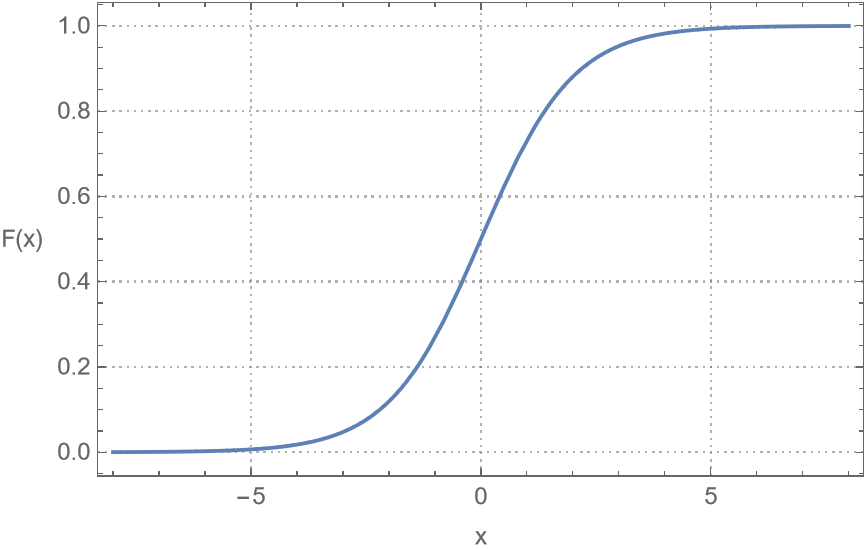
\includegraphics[width=0.4\linewidth]{sigmoide}
    \caption{Gráfica de la función sigmoide. Fuente: elaboración propia.}
    \label{fig:sigmoide}
  \end{figure}

\item \textbf{Tangente hiperbólica ($\tanh$):} su rango es $(-1,1)$. Es similar
  a la sigmoide pero centrada en el origen, lo que suele mejorar la
  convergencia. Su ecuación es
  \begin{equation}
    f(x)=\frac{e^{x}-e^{-x}}{e^{x}+e^{-x}}.
  \end{equation}

  \begin{figure}[H]
    \centering
    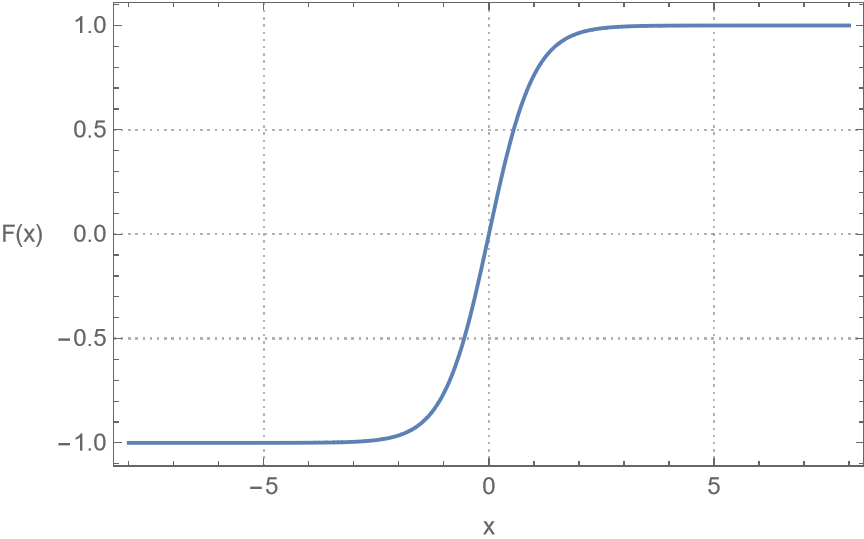
\includegraphics[width=0.4\linewidth]{tanh}
    \caption{Gráfica de la función tangente hiperbólica. Fuente: elaboración
      propia.}
    \label{fig:tanh}
  \end{figure}

\item \textbf{Rectificadora lineal (ReLU):} devuelve 0 para valores negativos y
  el valor original para valores positivos,
  \begin{equation}
    f(x)=\max(0,x).
  \end{equation}

  \begin{figure}[H]
    \centering
    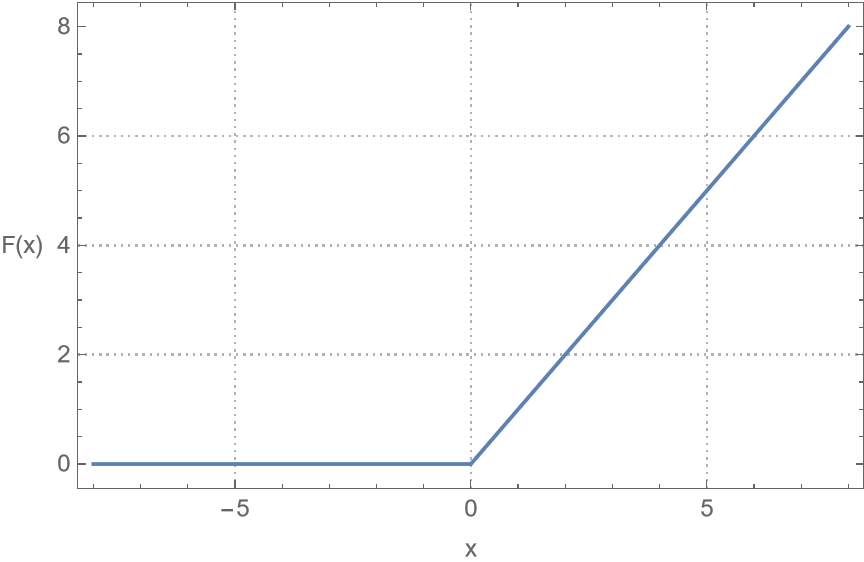
\includegraphics[width=0.4\linewidth]{relu}
    \caption{Gráfica de la función ReLU. Fuente: elaboración propia.}
    \label{fig:relu}
  \end{figure}

  La ReLU es barata de evaluar y su derivada no se satura para $x>0$, pero
  tiene un modo de falla conocido: si durante el entrenamiento el argumento de
  una neurona se vuelve negativo para todos los datos, su gradiente es cero de
  forma permanente y la neurona deja de aprender. Este fenómeno, llamado
  \emph{ReLU muerta}, es más probable cuanto menos neuronas tenga la capa, y se
  invocará en la sección~\ref{subsec:capacidad} para explicar el comportamiento
  de la red $\to2\to1$.
\end{enumerate}

\subsubsection{Función de coste}
\label{subsubsec:coste}
La función de coste mide el error entre el valor estimado y el valor real
durante el entrenamiento. Su minimización es el objetivo de todo el
proceso~\cite{antonio_2023_introduccin,ibm_qu}. Con $\hat y_i$ la predicción,
$y_i$ el valor real y $n$ el número de muestras:

\begin{enumerate}
\item \textbf{Error cuadrático medio (MSE):} es la función que se minimiza
  durante el entrenamiento,
  \begin{equation}
    \mathrm{MSE}=\frac{1}{n}\sum_{i=1}^{n}(\hat y_i-y_i)^2.
  \end{equation}

\item \textbf{Raíz del error cuadrático medio (RMSE):} es la raíz del anterior,
  \begin{equation}
    \mathrm{RMSE}=\sqrt{\frac{1}{n}\sum_{i=1}^{n}(\hat y_i-y_i)^2},
  \end{equation}
  con la ventaja de estar en las mismas unidades que la variable predicha ---
  metros, en este trabajo. Penaliza fuertemente los errores grandes.

\item \textbf{Error absoluto medio (MAE):} promedia los valores absolutos de
  los errores,
  \begin{equation}
    \mathrm{MAE}=\frac{1}{n}\sum_{i=1}^{n}\abs{\hat y_i-y_i}.
  \end{equation}
  Es más fácil de interpretar que el RMSE y menos sensible a valores atípicos.
\end{enumerate}

Un punto que conviene subrayar, porque organiza la presentación de los
resultados: MSE, RMSE y MAE son medidas \emph{relativas}. Un RMSE de
\num{0.5}~\meter\ es excelente si los datos varían en decenas de metros y es
pésimo si varían en centímetros. Por eso todo RMSE reportado aquí se acompaña
del $R^2$ de la ecuación~\eqref{eq:r2} y de las líneas base clásicas de la
sección~\ref{subsec:baselines}.

Además, existen optimizadores que usan estas funciones de coste para ajustar
los pesos:
\begin{itemize}
\item \textbf{Descenso estocástico del gradiente (SGD):} actualiza los pesos en
  la dirección opuesta al gradiente estimado sobre un subconjunto (lote) de los
  datos, $w \leftarrow w - \eta\,\partial C/\partial w$, con $\eta$ la tasa de
  aprendizaje.
\item \textbf{Adam:} adapta la tasa de aprendizaje de cada parámetro usando
  estimaciones del primer y segundo momento del gradiente. Es el optimizador
  empleado en todos los entrenamientos de este trabajo.
\end{itemize}

\subsection{Aprendizaje automático}
\label{subsec:ML}

\subsubsection{Backpropagation}
El \emph{backpropagation}, o propagación hacia atrás de errores, es el
algoritmo fundamental del aprendizaje supervisado en redes neuronales. Su
objetivo es ajustar los pesos para minimizar el error entre las predicciones y
los valores reales, y consiste en aplicar la regla de la
cadena~\eqref{eq:cadena} desde la salida hacia la entrada: se calcula el error
en la capa de salida, se propaga hacia atrás capa por capa multiplicando por
las derivadas locales, y con las derivadas parciales resultantes
$\partial C/\partial w$ el optimizador actualiza cada peso. El ciclo completo
sobre todo el conjunto de entrenamiento es una \emph{época}.

\subsubsection{Sobreajuste y validación}
\label{subsubsec:sobreajuste}
Entrenar durante muchas épocas puede llevar a que la red memorice
particularidades del conjunto de entrenamiento en lugar de aprender la
regularidad subyacente. Para detectarlo se separan los datos en un conjunto de
entrenamiento y uno de validación, y se vigila que el error de validación no
empiece a crecer mientras el de entrenamiento sigue bajando.

La forma en que se hace esa separación importa tanto como el hecho de hacerla.
Si los datos provienen de experimentos repetidos, repartir los puntos
individuales al azar hace que puntos de una misma trayectoria caigan a ambos
lados de la partición; entonces el conjunto de validación no mide capacidad de
generalización a un experimento nuevo, sino solo de interpolación dentro de
experimentos ya vistos. La alternativa correcta, y la que se emplea en este
trabajo, es particionar por \emph{experimento completo}: cada clip entra
íntegro en entrenamiento, en validación o en prueba, y nunca se reparte entre
ellos.

\subsubsection{Identificabilidad del modelo}
\label{subsubsec:identificabilidad}
Existe una condición previa a cualquier consideración de arquitectura o de
entrenamiento, y es que el problema planteado tenga solución. Si se busca una
función $f$ tal que $y\approx f(x)$ y en los datos existen pares $(x,y_a)$ y
$(x,y_b)$ con $y_a\neq y_b$, ninguna función puede reproducir ambos: el
problema es \emph{no identificable} a partir de $x$.

En ese caso la teoría de la regresión da una respuesta precisa. El minimizador
del error cuadrático esperado es la media condicional,
\begin{equation}
  f^{\star}(x)=\mathbb{E}[\,y\mid x\,],
  \label{eq:mediacondicional}
\end{equation}
y el error residual mínimo alcanzable es la varianza condicional
$\mathbb{E}[\operatorname{Var}(y\mid x)]$, que no puede reducirse por más
capacidad o más épocas que se le den al modelo. Una red suficientemente
expresiva entrenada con MSE converge a~\eqref{eq:mediacondicional}, no
necesariamente a la ley física que generó los datos.

Esta es la consideración que gobierna el diseño experimental de la
sección~\ref{subsec:formulaciones}. Aplicada a la caída libre dice lo
siguiente: si a la red se le da como única entrada el tiempo~$t$ del video y se
le pide la posición~$y$, un mismo $t$ queda asociado a las posiciones de
muchas trayectorias distintas, con alturas iniciales distintas, y la media
condicional resultante no tiene por qué parecerse a ninguna parábola física.
Para que la pregunta tenga respuesta, las entradas deben determinar la salida,
y eso obliga a construirlas de manera que la información propia de cada
trayectoria esté presente.

\subsection{PyTorch}
\label{subsec:ts}
El anteproyecto contemplaba usar TensorFlow~\cite{TensorFlow}, la plataforma de
aprendizaje automático desarrollada por Google y liberada en 2015. Durante la
implementación se migró a \textbf{PyTorch}, biblioteca de código abierto
mantenida por Meta AI, por dos razones prácticas: su modo de ejecución
inmediata (\emph{eager}) permite inspeccionar tensores y gradientes con un
depurador convencional, lo que resultó decisivo para un proyecto cuyo objetivo
es \emph{estudiar} el interior de la red y no solo entrenarla; y su API de
módulos (\texttt{torch.nn}) expresa arquitecturas pequeñas y no estándar con
menos código intermedio. Ambas bibliotecas implementan diferenciación
automática sobre grafos de cómputo y son equivalentes para los fines de este
trabajo. Los conceptos descritos en las secciones anteriores --- capas
lineales, activaciones, función de coste, optimizador Adam --- se traducen
directamente a las clases \texttt{nn.Linear}, \texttt{nn.ReLU}/\texttt{nn.Tanh},
\texttt{nn.MSELoss} y \texttt{torch.optim.Adam}.

El entorno de trabajo se gestionó con \texttt{conda} (entorno
\texttt{practicas}) y todos los scripts, datos y salidas quedaron versionados
en el repositorio del proyecto.


% % % % % % % % % % % % % % % % % % % % % % % % % % % % % % % % % % %
\section{Objetivos}
\label{sec:objetivos}

\subsection{General}
\label{sec:general}
\begin{itemize}
\item Estudiar la teoría, ejercicios, experiencias e historia del aprendizaje
  automático para entender la estructura interna de las redes neuronales
  aplicadas a la elaboración de modelos matemáticos que describan el
  comportamiento de los datos de montajes experimentales de caída libre.
\end{itemize}

\subsection{Específicos}
\label{sec:especificos}
\begin{itemize}
\item Estudiar el desarrollo histórico y aplicaciones del aprendizaje
  automático para la física.
\item Entender el funcionamiento de las redes neuronales de aprendizaje
  automático.
\item Construir redes neuronales básicas y entrenarlas.
\item Entrenar una red neuronal con ejemplos de MRUV.
\end{itemize}


% % % % % % % % % % % % % % % % % % % % % % % % % % % % % % % % % % %
\section{Justificación}
\label{sec:justificacion}
Las redes neuronales y los sistemas de aprendizaje automático están cada día
más presentes en la sociedad. Estas herramientas, a pesar de ser el foco de
discusiones éticas y morales, son de gran ayuda en diversas áreas: artísticas,
de productividad, financieras y, en especial, científicas. Las herramientas de
aprendizaje automático permiten la resolución de tareas complejas en segundos.
Además, se ha demostrado que son muy buenas al momento de buscar patrones y
crear \enquote{modelos} matemáticos, ya que en esencia su construcción es
matemática.

Tomando esto en cuenta, la idea es familiarizarse con la estructura,
entrenamiento y aspectos técnicos de las redes neuronales, para posteriormente
estudiar el modelo que utiliza la red para reproducir los resultados
experimentales. Una vez terminado, se tendrá una herramienta que puede ayudar
en la didáctica y divulgación de la ciencia y la tecnología.

Se espera que esto siente las bases para el Ejercicio de Práctica Supervisada
(EPS), que pretende seguir con este estudio y generalizar algunos aspectos para
diferentes marcos teóricos.

La motivación personal es adquirir experiencia en áreas de interés personal,
como lo son la física, la tecnología y la programación. Esto será una ayuda
para desenvolverme en la industria o en el mundo académico, según sea el caso,
sin desaprovechar la oportunidad de contribuir con la investigación nacional y
el desarrollo tecnológico y científico de Guatemala.


% % % % % % % % % % % % % % % % % % % % % % % % % % % % % % % % % % %
\section{Metodología}
\label{sec:metodologia}

El proyecto se desarrolló en cuatro etapas: estudio bibliográfico de redes
neuronales, montaje y digitalización del experimento de caída libre,
implementación y entrenamiento de las arquitecturas, y análisis de las redes
entrenadas. Las tres últimas se detallan a continuación.

\subsection{Montaje experimental y toma de datos}
\label{sec:datos}

Se grabaron \textbf{609 clips} de video de un cuerpo dejándose caer desde el
reposo, a una frecuencia de \unit{60}{\hertz} ($\Delta t = \unit{1/60}{\second}
\approx \unit{16.7}{\milli\second}$). Cada video se segmentó en clips
individuales y se digitalizó con \emph{Tracker}, obteniendo para cada
fotograma la tupla $(t,x,y,v_x,v_y,a_x,a_y)$; las velocidades y aceleraciones
son derivadas numéricas que el propio programa calcula por diferencias finitas
sobre las posiciones. La escala espacial se fijó con una referencia de longitud
conocida en el campo de visión, de modo que las posiciones están en metros y el
eje $y$ apunta hacia arriba.

De los 609 clips, \textbf{606 contienen datos utilizables}, con un total de
\textbf{\num{20\,210} pares $(t,y)$}. Cada clip tiene en promedio 33 puntos y una
duración media de \unit{0.54}{\second}. Los archivos resultantes se almacenaron
en formato de texto en \texttt{Toma\_de\_datos/datos/}.

\subsection{Preprocesamiento}
\label{subsec:preproceso}

Cada clip se refiere a su propio origen: con $t_0$ e $y_0$ el instante y la
posición del primer fotograma del clip, se definen
\begin{equation}
  \tau = t - t_0, \qquad \Delta y = y - y_0 ,
\end{equation}
de modo que la ecuación~\eqref{eq:mruv} se convierte en
\begin{equation}
  \Delta y = v_0\,\tau + \frac{1}{2}g\,\tau^2 .
  \label{eq:mruv_ref}
\end{equation}
En esta forma $y_0$ ha desaparecido y $g$ es el único parámetro compartido por
todas las trayectorias. La velocidad inicial $v_0$, en cambio, no es la misma
en todos los clips ---media $\num{-0.21}~\meter\per\second$, desviación
estándar $\num{0.25}~\meter\per\second$--- porque no todos empiezan en el
instante exacto de la soltada, y por eso se conserva como variable. Se estima
con un ajuste lineal a los \emph{tres primeros puntos} de cada clip:
\emph{Tracker} no proporciona velocidad en el primer fotograma, y usar solo el
arranque evita que la estimación absorba la curvatura, que es justamente lo que
se quiere medir después.

\paragraph{Filtro de calidad.} Se descartan los clips cuyo ajuste parabólico
deja un residuo superior a \unit{8}{\centi\meter}, que corresponden a fallos de
seguimiento de \emph{Tracker} ---el marcador salta de objeto o se pierde--- y
no a trayectorias físicamente distintas. El filtro elimina 25 de los 606 clips
(\SI{4}{\percent}) y deja \textbf{581 clips con \num{18\,992} muestras}.

\paragraph{Partición.} Los clips completos se reparten en
\SI{70}{\percent}/\SI{15}{\percent}/\SI{15}{\percent} para entrenamiento,
validación y prueba (407/87/87 clips), siguiendo el criterio de la
sección~\ref{subsubsec:sobreajuste}. La normalización $z$ de la
ecuación~\eqref{eq:zscore} se ajusta únicamente con los clips de
entrenamiento.

\subsection{Formulaciones evaluadas}
\label{subsec:formulaciones}

La sección~\ref{subsubsec:identificabilidad} indica que la elección de las
entradas no es un detalle de implementación sino la condición que determina si
el problema tiene solución. Para medir el efecto de cada ingrediente en lugar
de darlo por supuesto, se evaluaron tres formulaciones:

\begin{description}
\item[Directa, $t\to y$.] La red recibe el tiempo del video y devuelve la
  posición, con todos los clips concatenados. Es la formulación más ingenua
  posible y sirve de control: según el análisis de identificabilidad, un mismo
  $t$ está asociado a posiciones de clips distintos y el problema no queda
  determinado.
\item[Referida, $\tau\to\Delta y$.] Solo el cambio de origen de la
  ecuación~\eqref{eq:mruv_ref}. Mide cuánto se gana con eliminar $y_0$.
\item[Completa, $(\tau,v_0)\to\Delta y$.] Formulación identificable: las dos
  entradas determinan la salida a través de~\eqref{eq:mruv_ref}, con $g$ como
  único parámetro por aprender.
\end{description}

\subsection{Arquitecturas evaluadas}
\label{subsec:arquitecturas}

Se compararon tres configuraciones, elegidas para cubrir un rango amplio de
capacidad expresiva con el mismo conjunto de entradas:

\begin{itemize}
\item \textbf{Red simple $\to2\to1$.} Una capa oculta de dos neuronas con
  activación ReLU (7--9 parámetros según la formulación). Es la prueba más
  exigente.
\item \textbf{Red media $\to4\to1$.} Una capa oculta de cuatro neuronas con
  activación ReLU (13--17 parámetros).
\item \textbf{Red $\tanh$ profunda $\to32\to32\to1$.} Dos capas ocultas de 32
  neuronas con activación $\tanh$ (unos \num{1150} parámetros). Tiene capacidad
  expresiva muy superior a las anteriores.
\end{itemize}

Las tres se entrenaron con optimizador Adam, tasa de aprendizaje $10^{-2}$,
función de coste MSE sobre los datos normalizados, hasta 800 épocas y con
parada temprana sobre los clips de validación. Cada combinación de formulación
y arquitectura se repitió con \textbf{cinco semillas} distintas, en total
\textbf{45 entrenamientos}, y todos los resultados se reportan como media y
desviación estándar sobre esas semillas.

\subsection{Líneas base}
\label{subsec:baselines}

Un RMSE aislado no significa nada, de modo que se comparó contra tres
referencias clásicas, de la más débil a la más fuerte:

\begin{enumerate}
\item \textbf{Predictor constante.} Devuelve siempre la media de los datos. Su
  RMSE es, por construcción, la desviación estándar del conjunto. Es el mínimo
  que cualquier modelo debe superar holgadamente.
\item \textbf{MRUV con $g$ global.} Se estima una única $g$ con los clips de
  entrenamiento y se predice $\Delta y = v_0\tau+\tfrac{1}{2}g\tau^2$ en los
  clips de prueba. Es la ecuación de la física con \emph{un solo parámetro
  ajustado}, y es el rival de verdad: una red con cientos de parámetros que no
  lo iguale no está aportando nada.
\item \textbf{Ajuste parabólico por clip (oráculo).} Ajusta cada clip de prueba
  por separado, con tres parámetros libres \emph{por clip}. No es un predictor
  honesto, porque usa el propio clip que evalúa, pero marca el suelo de error
  alcanzable: lo que queda por debajo es ruido de medición.
\end{enumerate}

\subsection{Protocolo de evaluación}
\label{sec:protocolo}

El desempeño se evaluó siempre sobre \emph{clips que la red no vio durante el
entrenamiento}, y en dos niveles.

\paragraph{Nivel 1: error de predicción.} RMSE y MAE sobre la posición
desnormalizada, en metros, y el coeficiente de determinación $R^2$ de la
ecuación~\eqref{eq:r2} para situar esos errores frente a la dispersión propia
de los datos y frente a las líneas base.

\paragraph{Nivel 2: recuperación del parámetro físico.} Se ajusta la parábola
de la sección~\ref{subsubsec:minimoscuadrados} a las predicciones de la red
\emph{para cada clip de prueba por separado} y se toma $g=2c_2$; el resultado
del nivel 2 es la mediana de esas estimaciones. El mismo procedimiento aplicado
a los datos experimentales da el valor de referencia. Como se advirtió en la
sección~\ref{subsubsec:minimoscuadrados}, el ajuste debe hacerse clip por clip:
un ajuste único sobre los puntos de todos los clips agregados mezcla
trayectorias con distinto origen y distinta altura inicial, y su coeficiente
cuadrático no es $g/2$ sino un número sin interpretación física.

Este segundo nivel es el que verifica el supuesto del anteproyecto: si una red
\enquote{entiende} el marco teórico de la caída libre debe aproximar bien la
posición y, además, entregar el valor correcto de $g$ al ajustarle una parábola
a sus predicciones.

\paragraph{Nivel 3: estructura interna.} Los dos niveles anteriores juzgan a la
red por sus salidas. Como el objetivo general del anteproyecto habla de
\emph{entender la estructura interna} de la red, se añadieron dos análisis más:

\begin{itemize}
\item Un \textbf{estudio del número de épocas}, que mide el tiempo acumulado de
  entrenamiento, el RMSE y la $g$ recuperada en puntos de control a lo largo de
  un mismo entrenamiento, para valorar el coste y el beneficio de entrenar más
  (sección~\ref{subsec:epocas}).
\item Una \textbf{inspección de la red entrenada}, que escribe explícitamente
  la función de la red pequeña, calcula por diferenciación automática las
  derivadas de la función aprendida por la red $\tanh$ y las contrasta con las
  que exige la ecuación~\eqref{eq:mruv_ref}, y examina los pesos de la primera
  capa (sección~\ref{subsec:pesos}).
\end{itemize}


% % % % % % % % % % % % % % % % % % % % % % % % % % % % % % % % % % %
\section{Resultados}
\label{sec:resultados}

\subsection{Caracterización del conjunto de datos}
\label{subsec:datos_res}

Antes de evaluar ninguna red conviene establecer qué física contienen los
datos, porque \textbf{ningún modelo puede recuperar más de lo que hay en el
conjunto}. La tabla~\ref{tab:datos} resume las propiedades del conjunto antes y
después del filtro de calidad.

\begin{table}[H]
  \centering
  \begin{tabular}{lrr}
    \toprule
    & Sin filtro & Con filtro \\
    \midrule
    Clips                          & 606    & 581 \\
    Muestras $(t,y)$               & \num{20\,210} & \num{18\,992} \\
    Duración media [\second]       & 0.539  & 0.528 \\
    Puntos por clip (media)        & 33.3   & 32.7 \\
    $v_0$ media [\meter\per\second] & $-0.213$ & $-0.205$ \\
    $v_0$ desv.\ est.\ [\meter\per\second] & 0.265 & 0.247 \\
    \midrule
    $g$ por clip, mediana [\meter\per\second\squared] & $-9.378$ & $\mathbf{-9.426}$ \\
    $g$ por clip, desv.\ est.\ [\meter\per\second\squared] & 2.357 & 1.817 \\
    Residuo del ajuste, mediana [\meter] & 0.0350 & 0.0343 \\
    \bottomrule
  \end{tabular}
  \caption{Propiedades del conjunto experimental antes y después de descartar
    los clips con residuo del ajuste superior a \unit{8}{\centi\meter}. La $g$
    por clip se obtiene ajustando una parábola independiente a cada
    trayectoria.}
  \label{tab:datos}
\end{table}

El montaje experimental supera la prueba: el ajuste clásico clip por clip da
\begin{equation}
  g_{\text{exp}} = \num{-9.43}~\meter\per\second\squared ,
  \label{eq:gexp}
\end{equation}
a un \SI{3.9}{\percent} del valor físico $\num{-9.81}~\meter\per\second\squared$.
La información física \emph{está presente en los datos}. Esa diferencia del
\SI{3.9}{\percent} es un sesgo del experimento ---probablemente de calibración
de la escala espacial o de la velocidad de fotogramas declarada--- y afecta por
igual a la red y a cualquier método clásico, de modo que el criterio de éxito
para la red es acercarse a $g_{\text{exp}}$, no a $\num{-9.81}$.

La dispersión de $\num{1.82}~\meter\per\second\squared$ entre clips se atribuye
a la corta duración de cada uno ---media \unit{0.53}{\second}, unos 33
puntos--- combinada con la resolución espacial del seguimiento; el residuo
mediano del ajuste, \unit{3.4}{\centi\meter}, marca el suelo de ruido del
conjunto. La figura~\ref{fig:datos} muestra unos cuantos clips ya referidos a
su propio origen y la distribución completa de las 581 estimaciones de $g$.

\begin{figure}[H]
  \centering
  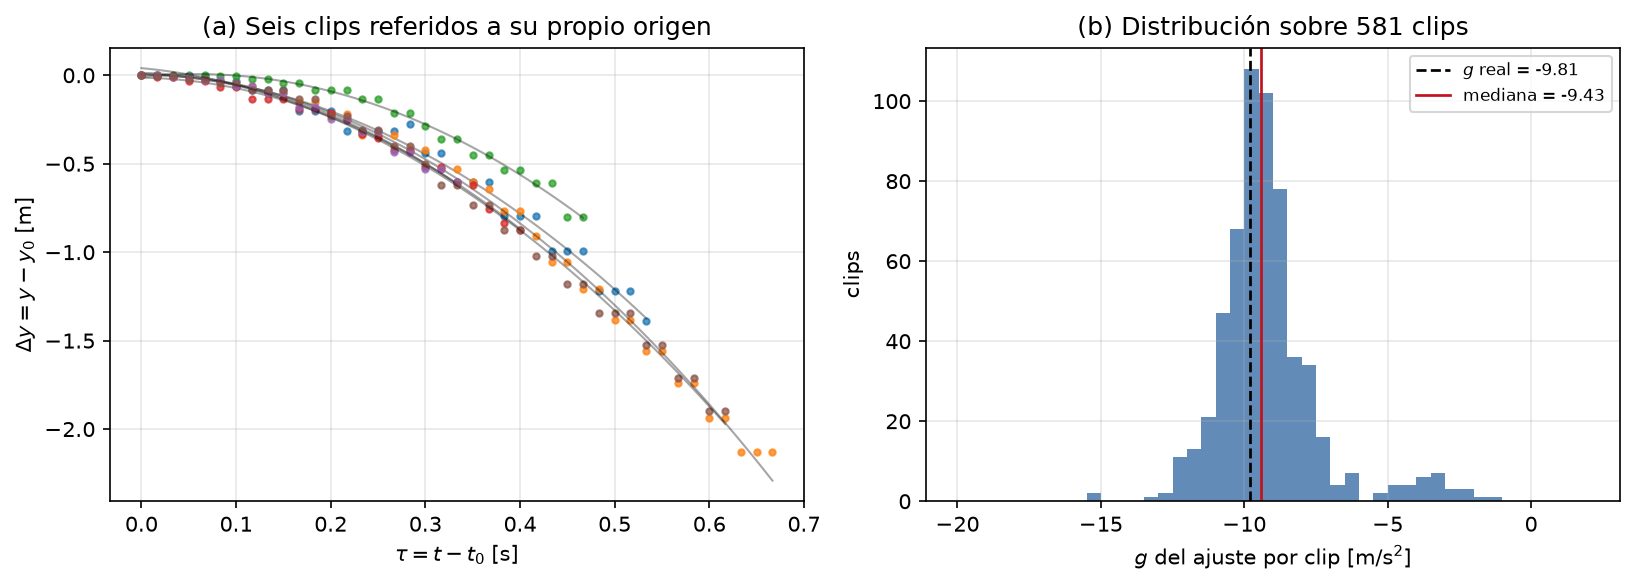
\includegraphics[width=\linewidth]{imgs/00_datos.png}
  \caption{(a) Seis clips experimentales referidos a su propio origen, con su
    ajuste parabólico. Bajo esta representación todas las trayectorias arrancan
    en el mismo punto y comparten la misma curvatura, que es lo que fija $g$.
    (b) Distribución de la $g$ obtenida ajustando una parábola a cada uno de
    los 581 clips; la mediana está a un \SI{3.9}{\percent} del valor físico.}
  \label{fig:datos}
\end{figure}

\subsection{Recuperación del parámetro físico}
\label{subsec:g}

La tabla~\ref{tab:g} recoge el resultado principal del trabajo.

\begin{table}[H]
  \centering
  \begin{tabular}{llrrr}
    \toprule
    Formulación & Arquitectura & Parámetros & $g$ recuperada & Error vs.\ $-9.81$ \\
    \midrule
    \multirow{3}{*}{Directa}
      & simple $(2)$    & 7    & $+0.00 \pm 0.00$ & \SI{100.0}{\percent} \\
      & media $(4)$     & 13   & $-1.21 \pm 1.67$ & \SI{87.6}{\percent} \\
      & tanh $32\times32$ & 1153 & $-2.77 \pm 0.56$ & \SI{71.8}{\percent} \\
    \midrule
    \multirow{3}{*}{Referida}
      & simple $(2)$    & 7    & $-3.02 \pm 4.14$ & \SI{69.2}{\percent} \\
      & media $(4)$     & 13   & $-7.61 \pm 0.39$ & \SI{22.5}{\percent} \\
      & tanh $32\times32$ & 1153 & $-9.07 \pm 0.28$ & \SI{7.6}{\percent} \\
    \midrule
    \multirow{3}{*}{Completa}
      & simple $(2)$    & 9    & $-4.68 \pm 4.30$ & \SI{52.3}{\percent} \\
      & media $(4)$     & 17   & $-7.53 \pm 0.57$ & \SI{23.3}{\percent} \\
      & \textbf{tanh $32\times32$} & 1185 & $\mathbf{-9.46 \pm 0.33}$
        & \textbf{\SI{3.8}{\percent}} \\
    \midrule
    \multicolumn{3}{l}{\emph{Referencia experimental} (ajuste por clip)}
      & $-9.48 \pm 0.11$ & \SI{3.4}{\percent} \\
    \bottomrule
  \end{tabular}
  \caption{Mediana de la $g$ recuperada ajustando una parábola a las
    predicciones de cada clip de prueba, en \meter\per\second\squared. Media y
    desviación estándar sobre cinco semillas, evaluadas siempre sobre clips que
    la red no vio durante el entrenamiento.}
  \label{tab:g}
\end{table}

El resultado es inequívoco. Con la formulación completa, la red $\tanh$
profunda recupera
\begin{equation}
  g = \num{-9.46} \pm \num{0.33}~\meter\per\second\squared .
\end{equation}
La comparación pertinente no es contra $\num{-9.81}$ sino contra la referencia
experimental $\num{-9.48}~\meter\per\second\squared$, que es lo que el método
clásico extrae de estos mismos clips de prueba: la discrepancia es entonces de
\textbf{\SI{0.2}{\percent}}. La red reproduce la gravedad contenida en el
conjunto de datos prácticamente sin sesgo; el \SI{3.4}{\percent} restante
frente al valor verdadero es la limitación del experimento discutida en la
sección~\ref{subsec:datos_res}, común a la red y al método clásico.

La figura~\ref{fig:form} presenta el mismo resultado gráficamente, y la
figura~\ref{fig:hist} muestra las distribuciones completas: bajo la formulación
directa las estimaciones de la red y las de los datos forman dos poblaciones
separadas, mientras que bajo la formulación completa se superponen.

\begin{figure}[H]
  \centering
  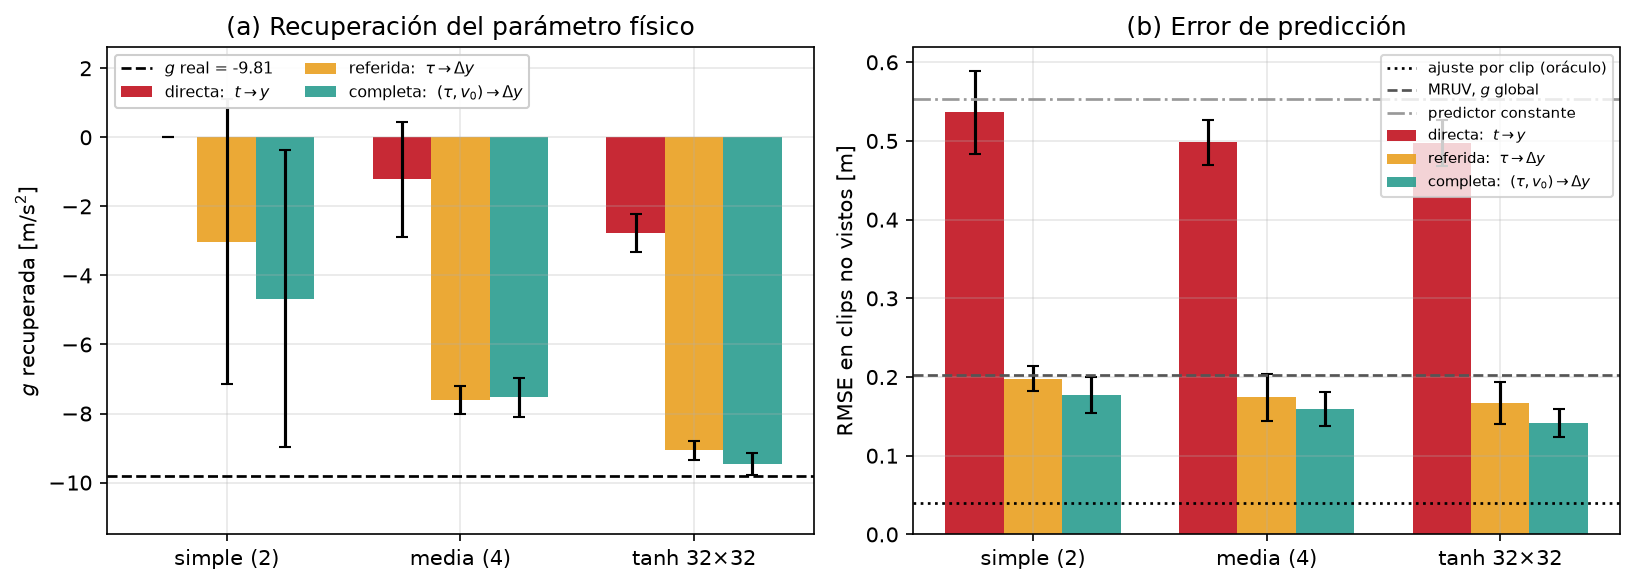
\includegraphics[width=\linewidth]{imgs/01_formulaciones.png}
  \caption{(a) Gravedad recuperada por formulación y arquitectura; la línea
    discontinua es el valor físico. (b) RMSE sobre clips no vistos, con las
    tres líneas base como referencia. Barras de error: desviación estándar
    sobre cinco semillas.}
  \label{fig:form}
\end{figure}

\begin{figure}[H]
  \centering
  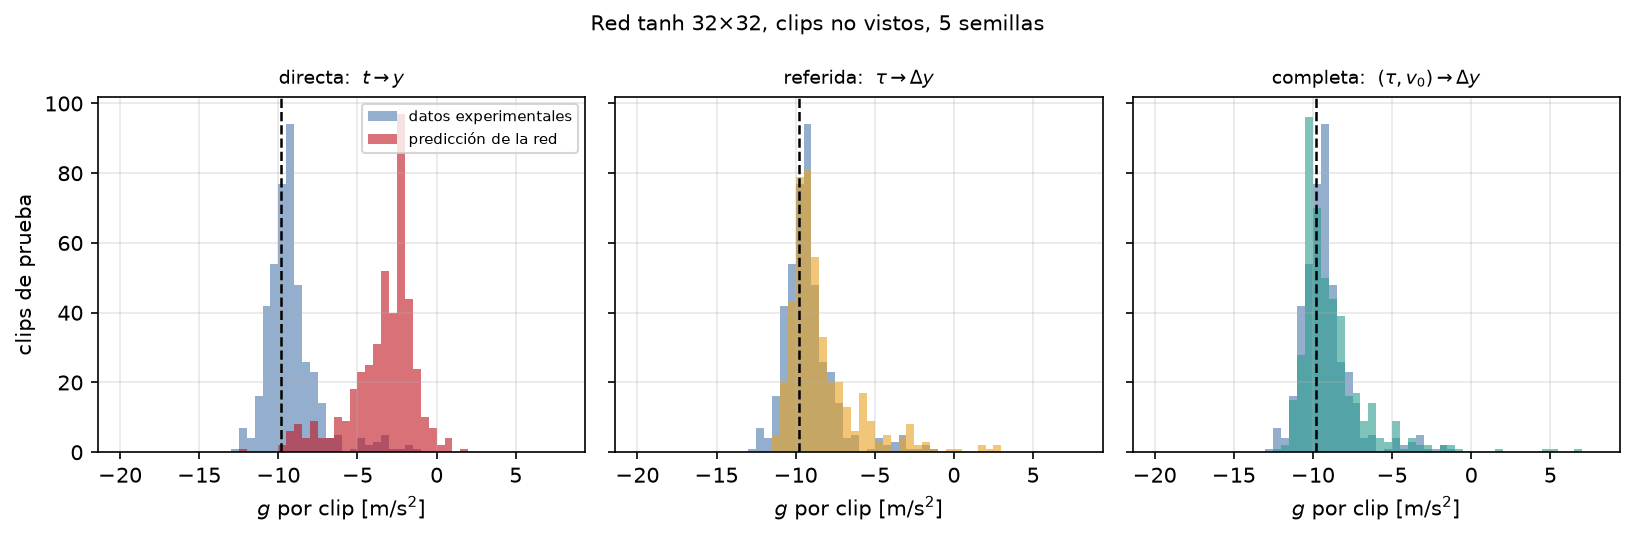
\includegraphics[width=\linewidth]{imgs/02_g_por_clip.png}
  \caption{Distribución de la $g$ estimada clip por clip para la red
    $\tanh$ $32\times32$; en azul la de los datos experimentales y en color la
    de las predicciones. Al pasar de la formulación directa a la completa las
    dos distribuciones dejan de estar separadas y se superponen.}
  \label{fig:hist}
\end{figure}

La figura~\ref{fig:tray} es quizá la más ilustrativa del informe, porque
muestra el mecanismo. Con la formulación directa la red produce prácticamente
la misma curva para los cuatro clips ---no puede hacer otra cosa, porque su
única entrada $t$ no distingue un clip de otro--- y los desajustes llegan a un
metro. Con la formulación completa, la misma arquitectura sigue la parábola de
cada clip.

\begin{figure}[H]
  \centering
  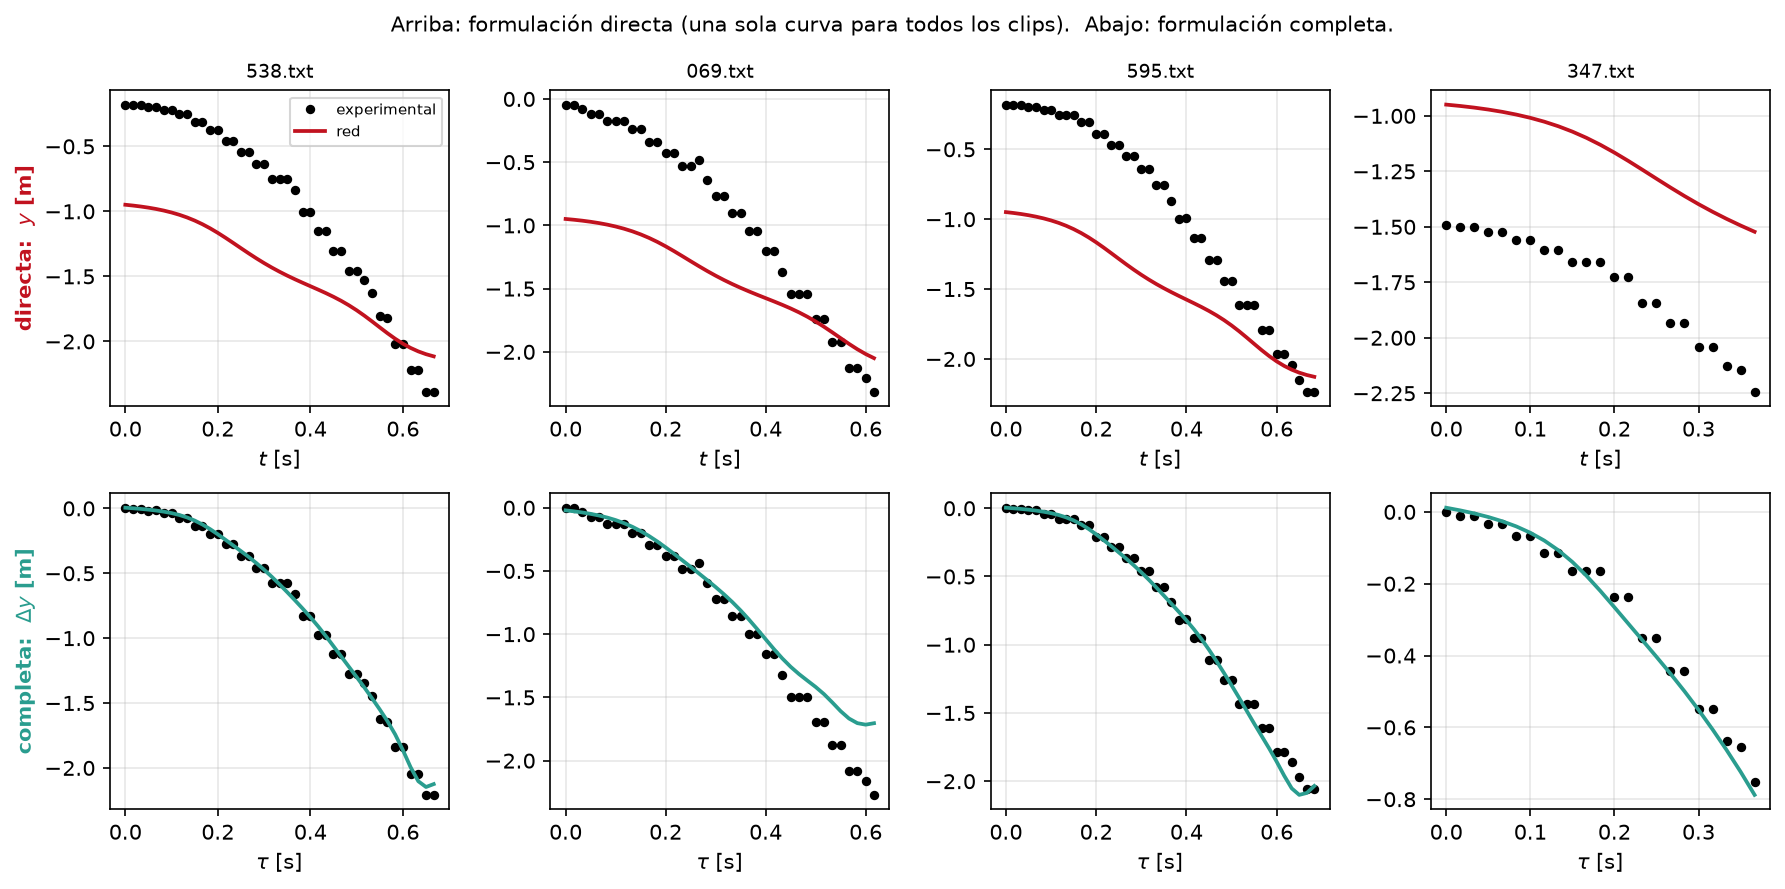
\includegraphics[width=\linewidth]{imgs/03_trayectorias.png}
  \caption{Cuatro clips de prueba con las predicciones de la red
    $\tanh$ $32\times32$. Arriba, formulación directa: la red no puede
    distinguir un clip de otro y predice esencialmente la misma curva para
    todos. Abajo, formulación completa: la red reproduce la trayectoria de cada
    clip.}
  \label{fig:tray}
\end{figure}

\subsection{Error de predicción}
\label{subsec:error}

La tabla~\ref{tab:rmse} sitúa el error de predicción de la red frente a las
tres líneas base de la sección~\ref{subsec:baselines}.

\begin{table}[H]
  \centering
  \begin{tabular}{lrrr}
    \toprule
    Modelo & RMSE [\meter] & MAE [\meter] & $R^2$ \\
    \midrule
    Predictor constante $\bar y$              & 0.5534 & --- & 0.000 \\
    Red directa, $\tanh$ $32\times32$         & 0.4970 & 0.4170 & 0.329 \\
    \midrule
    MRUV con $g$ global (1 parámetro)         & 0.2020 & 0.0841 & 0.841 \\
    Red referida, $\tanh$ $32\times32$        & 0.1670 & 0.0984 & 0.898 \\
    \textbf{Red completa, $\tanh$ $32\times32$} & \textbf{0.1420}
      & \textbf{0.0728} & \textbf{0.926} \\
    \midrule
    Ajuste por clip (oráculo, 3 parám./clip)  & 0.0401 & 0.0286 & 0.994 \\
    Suelo de ruido (residuo del ajuste)       & 0.0343 & --- & --- \\
    \bottomrule
  \end{tabular}
  \caption{Error de predicción sobre clips no vistos, promediado sobre cinco
    semillas. Todas las cantidades en metros.}
  \label{tab:rmse}
\end{table}

Tres observaciones.

\paragraph{La red explica el \SI{93}{\percent} de la varianza.} Con la
formulación completa el RMSE es de \num{0.142}~\meter\ y el $R^2$ de
\num{0.93}, frente a los \num{0.553}~\meter\ del predictor constante. La
formulación directa se queda en $R^2=\num{0.33}$: capta un tercio de la
estructura de los datos, que es lo que cabe esperar de un modelo cuya entrada
no determina la salida.

\paragraph{La red supera al modelo físico analítico.} La ecuación de MRUV con
$g$ global alcanza RMSE~$=\num{0.202}~\meter$; la red llega a
$\num{0.142}~\meter$, un \SI{30}{\percent} mejor \emph{con las mismas
entradas}. La razón más probable es que $v_0$, estimado a partir de tres puntos
ruidosos, arrastra un sesgo sistemático que la red aprende a compensar y que la
fórmula analítica no puede corregir. Este es el punto del proyecto en el que la
red aporta algo que el método clásico no da.

\paragraph{Aún queda margen.} El oráculo por clip alcanza
$\num{0.040}~\meter$, cerca del suelo de ruido de $\num{0.034}~\meter$. La
diferencia con los $\num{0.142}~\meter$ de la red se explica porque el oráculo
ajusta tres parámetros \emph{por clip}, mientras que la red dispone únicamente
de $(\tau,v_0)$ y no puede reproducir las desviaciones individuales de cada
trayectoria.

\subsection{Representación de las entradas y capacidad de la red}
\label{subsec:capacidad}

Hay un contraste en las tablas~\ref{tab:g} y~\ref{tab:rmse} que merece atención
propia, porque es el resultado más instructivo del estudio.

Bajo la formulación directa, pasar de 7 a \num{1153} parámetros ---un factor
165--- apenas cambia nada: el RMSE baja de \num{0.537} a \num{0.497}~\meter\ y
la $g$ recuperada sigue siendo inservible. Bajo la formulación completa, esa
misma escalada lleva la $g$ de $\num{-4.68}$ a $\num{-9.46}$ y el RMSE de
\num{0.177} a \num{0.142}~\meter.

Es decir: \textbf{mientras el problema no es identificable, la capacidad no
importa; una vez lo es, la capacidad pasa a ser el factor decisivo.} Eso es
exactamente lo que predice el análisis de la
sección~\ref{subsubsec:identificabilidad}. Cuando el límite es de
\emph{información}, ninguna arquitectura puede superarlo, porque la solución
óptima ---la media condicional--- ya está al alcance de una red pequeña. Cuando
el límite es de \emph{representación}, una red mayor sí ayuda.

El comportamiento de la red $\to2\to1$ bajo la formulación completa
($g=\num{-4.68}$, con una dispersión entre semillas de $\num{4.30}$) es una
limitación genuina de capacidad: dos unidades ReLU solo pueden formar una
función lineal a trozos con dos quiebres, con la que no se aproxima una
parábola. La inestabilidad entre semillas es coherente con el fenómeno de ReLU
muerta descrito en la sección~\ref{subsec:redneuronal}: basta con que una de las
dos unidades quede en la región de gradiente nulo para que la red se reduzca de
hecho a una sola neurona, y el resultado depende entonces críticamente de la
inicialización.

La figura~\ref{fig:scatter} resume las 45 corridas en un solo gráfico y hace
visible que ambos ejes ---error de predicción y error en $g$--- mejoran juntos,
pero que solo la combinación de formulación identificable y capacidad
suficiente baja del \SI{5}{\percent} de error en el parámetro físico.

\begin{figure}[H]
  \centering
  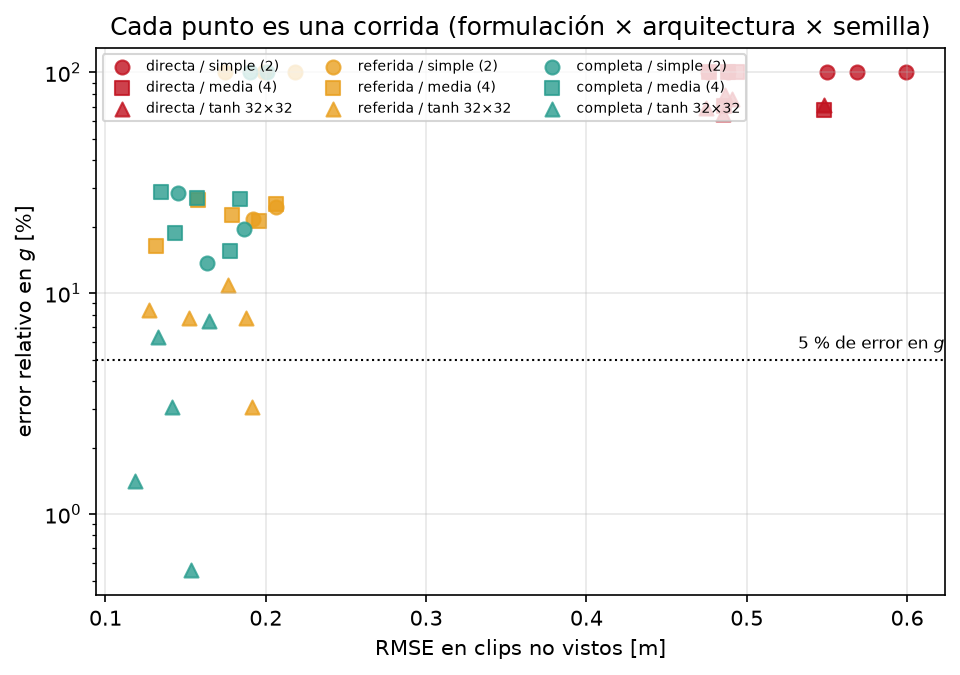
\includegraphics[width=0.78\linewidth]{imgs/04_rmse_vs_error_g.png}
  \caption{Error relativo en $g$ frente al RMSE para las 45 corridas
    (3 formulaciones $\times$ 3 arquitecturas $\times$ 5 semillas). Las corridas
    con la formulación directa se agrupan arriba a la derecha; solo la
    formulación completa con la red $\tanh$ profunda baja del
    \SI{5}{\percent} de error.}
  \label{fig:scatter}
\end{figure}

\subsection{Coste y beneficio del número de épocas}
\label{subsec:epocas}

Entrenar más épocas cuesta tiempo de cómputo. Para decidir cuánto conviene
gastar se entrenó cada arquitectura bajo la formulación completa evaluándola en
puntos de control a lo largo de un \emph{mismo} entrenamiento, de modo que el
tiempo reportado para la época $N$ es el tiempo real acumulado hasta llegar a
ella y la curva de error es una trayectoria de aprendizaje y no una colección
de entrenamientos independientes. La tabla~\ref{tab:epocas} y la
figura~\ref{fig:epocas} recogen el resultado, promediado sobre las cinco
semillas.

\begin{table}[H]
  \centering
  \begin{tabular}{lrrrrr}
    \toprule
    Arquitectura & Épocas & Tiempo [\second] & RMSE [\meter] & $R^2$
      & Error en $g$ \\
    \midrule
    \multirow{7}{*}{simple $(2)$}
      &   1 &  0.01 & 0.4999 & 0.095 & \SI{101.9}{\percent} \\
      &  10 &  0.09 & 0.2185 & 0.819 & \SI{54.4}{\percent} \\
      &  50 &  0.43 & 0.1783 & 0.884 & \SI{52.0}{\percent} \\
      & 100 &  0.85 & 0.1787 & 0.884 & \SI{53.6}{\percent} \\
      & 200 &  1.70 & 0.1782 & 0.884 & \SI{54.5}{\percent} \\
      & 400 &  3.39 & 0.1784 & 0.884 & \SI{54.0}{\percent} \\
      & 800 &  6.76 & 0.1775 & 0.885 & \SI{54.4}{\percent} \\
    \midrule
    \multirow{7}{*}{media $(4)$}
      &   1 &  0.01 & 0.4350 & 0.310 & \SI{92.1}{\percent} \\
      &  10 &  0.09 & 0.1670 & 0.898 & \SI{17.7}{\percent} \\
      &  50 &  0.43 & 0.1654 & 0.900 & \SI{20.9}{\percent} \\
      & 100 &  0.86 & 0.1602 & 0.906 & \SI{22.9}{\percent} \\
      & 200 &  1.70 & 0.1619 & 0.904 & \SI{28.4}{\percent} \\
      & 400 &  3.39 & 0.1593 & 0.908 & \SI{30.8}{\percent} \\
      & 800 &  6.79 & 0.1566 & 0.911 & \SI{29.1}{\percent} \\
    \midrule
    \multirow{7}{*}{$\tanh$ $32\times32$}
      &   1 &  0.01 & 0.2145 & 0.833 & \SI{74.5}{\percent} \\
      &  10 &  0.13 & 0.1519 & 0.916 & \SI{12.5}{\percent} \\
      &  50 &  0.65 & 0.1488 & 0.920 & \SI{7.2}{\percent} \\
      & 100 &  1.29 & 0.1441 & 0.925 & \SI{7.0}{\percent} \\
      & \textbf{200} & \textbf{2.57} & \textbf{0.1430} & \textbf{0.926}
        & \textbf{\SI{4.3}{\percent}} \\
      & 400 &  5.13 & 0.1459 & 0.923 & \SI{7.5}{\percent} \\
      & 800 & 10.27 & 0.1504 & 0.918 & \SI{6.2}{\percent} \\
    \bottomrule
  \end{tabular}
  \caption{Tiempo acumulado de entrenamiento, error de predicción sobre clips
    no vistos y error relativo en $g$ frente al número de épocas. Media sobre
    cinco semillas. El tiempo corresponde a un procesador de escritorio con
    cuatro hilos.}
  \label{tab:epocas}
\end{table}

\begin{figure}[H]
  \centering
  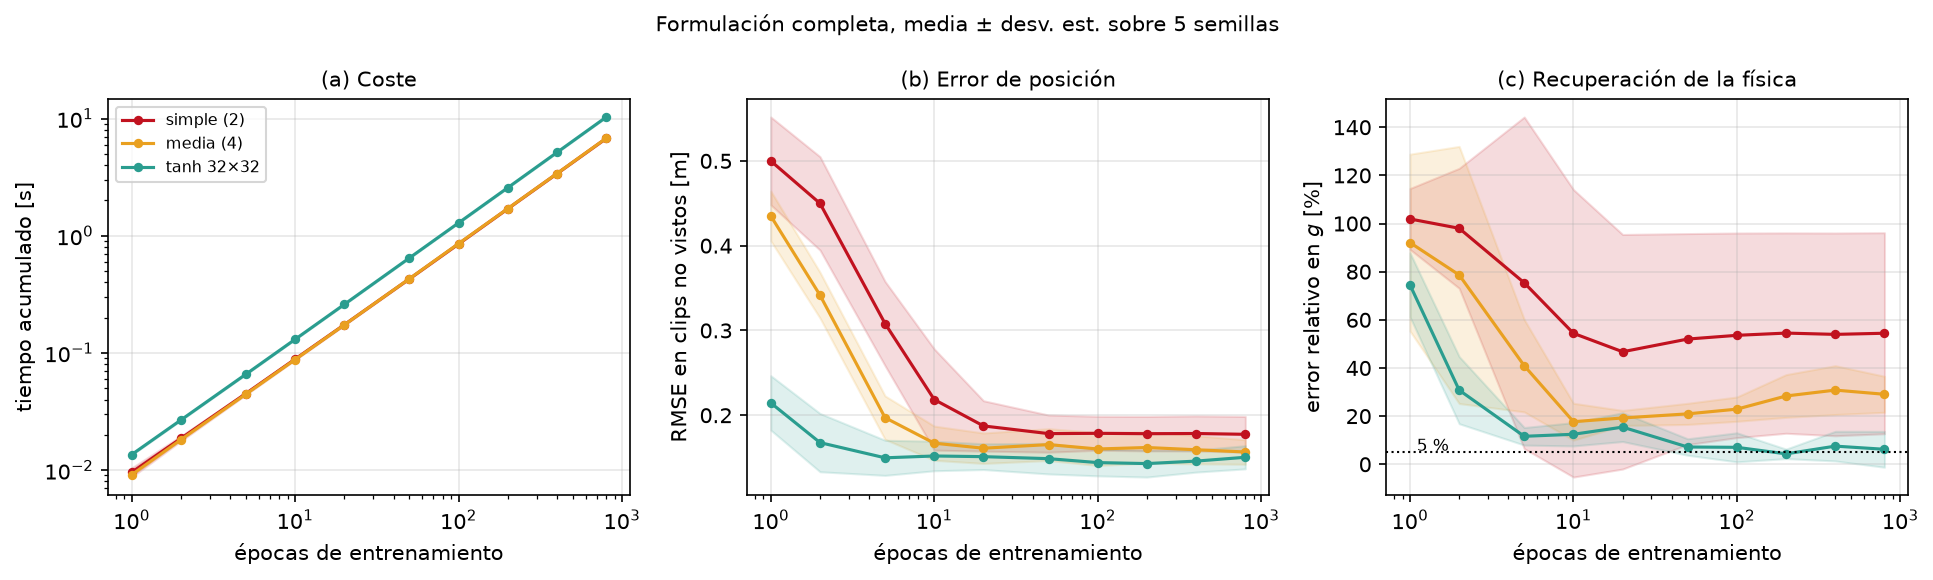
\includegraphics[width=\linewidth]{imgs/05_epocas.png}
  \caption{(a) Tiempo acumulado de entrenamiento, estrictamente lineal en el
    número de épocas. (b) RMSE sobre clips no vistos. (c) Error relativo en la
    $g$ recuperada. Bandas: desviación estándar sobre cinco semillas. Nótese
    que el eje de épocas es logarítmico: los tramos finales de las curvas
    cuestan la mayor parte del tiempo total.}
  \label{fig:epocas}
\end{figure}

Tres observaciones, y la tercera es la importante.

\paragraph{El coste es exactamente lineal.} El panel (a) de la
figura~\ref{fig:epocas} es una recta en escala doblemente logarítmica con
pendiente 1: cada época cuesta lo mismo que la anterior. Duplicar las épocas
duplica el tiempo, sin excepción. La red $\tanh$, con \num{1185} parámetros,
cuesta apenas un \SI{50}{\percent} más por época que las de 9 y 17: a estos
tamaños el coste lo domina el recorrido de los datos, no el número de
parámetros.

\paragraph{El error de posición se estanca muy pronto.} Las tres redes alcanzan
prácticamente su RMSE final hacia la época 10 o 20. De la época 50 a la 800 ---
un factor 16 en tiempo --- la red $\tanh$ mejora el RMSE en un
\SI{4}{\percent} y luego lo empeora. Juzgando solo por el RMSE, todo lo que se
entrene por encima de unas 50 épocas es tiempo perdido.

\paragraph{La física no aparece al mismo ritmo que baja el error, y puede
retroceder.} El panel (c) muestra un comportamiento que el RMSE no deja ver.
La red $\tanh$ necesita alrededor de 200 épocas para llegar a su mejor
estimación de $g$ (\SI{4.3}{\percent} de error), es decir, cuatro veces más
entrenamiento del que necesitaba para estabilizar el RMSE. Y la red media $(4)$
hace lo contrario: su RMSE mejora monótonamente de \num{0.167} a
\num{0.157}~\meter\ entre las épocas 10 y 800, mientras su error en $g$
\emph{empeora} de \SI{17.7}{\percent} a \SI{29.1}{\percent}. Sigue reduciendo
el error cuadrático, pero lo hace ajustando aspectos de los datos que no son la
curvatura.

Esto tiene una consecuencia práctica directa: \textbf{el criterio de parada no
puede basarse solo en el error de predicción} cuando lo que se busca es un
parámetro físico. Las dos cantidades no son monótonas entre sí. En este trabajo
la parada temprana sobre clips de validación completos (sección
\ref{subsec:arquitecturas}) restaura para la red $\tanh$ los pesos de la época
162 de media, con un rango de 41 a 275 entre semillas. El valor medio cae en la
ventana de 100--200 épocas donde la $g$ es mejor, pero la anchura de ese rango
indica que se trata de una coincidencia afortunada del problema y no de una
garantía general.

En cuanto a la pregunta de coste-beneficio: para esta red y estos datos, el
punto de operación razonable está entre 100 y 200 épocas, unos
\SI{1.3}{\second} a \SI{2.6}{\second} de cómputo. Las 600 épocas adicionales
hasta el límite de 800 multiplican por cuatro el tiempo, empeoran ligeramente
el RMSE y no mejoran la estimación de $g$.

\subsection{Inspección de la red entrenada}
\label{subsec:pesos}

El objetivo general del anteproyecto no era solo predecir bien, sino
\enquote{entender la estructura interna de las redes neuronales aplicadas a la
elaboración de modelos matemáticos}. Ajustar una parábola a las
\emph{salidas} de la red, como se hizo en la sección~\ref{subsec:g}, muestra
que la red se \emph{comporta} como la física; esta sección mira la función que
la red implementa, para ver si la física está además en su estructura.

\subsubsection{La red simple, escrita a mano}

Con 9 parámetros la función de la red $\to2\to1$ se puede escribir completa. En
unidades físicas, para la semilla 0:
\begin{align}
  h_0 &= \max(0,\; +0.082\,\tau + 0.830\,v_0 - 0.271), \nonumber\\
  h_1 &= \max(0,\; -4.530\,\tau + 0.410\,v_0 + 3.056), \label{eq:relu_explicita}\\
  \Delta y &= 0.006\,h_0 + 0.617\,h_1 - 1.585. \nonumber
\end{align}
Es una función lineal a trozos con dos quiebres. Su segunda derivada es cero en
todas partes salvo en los quiebres, donde no existe. No hay ningún valor de los
nueve parámetros que produzca la curvatura constante que se necesita para
representar $g$, lo que confirma por construcción ---y no por evidencia
estadística--- la limitación de capacidad de la sección~\ref{subsec:capacidad}.
Nótese además que la primera unidad llega a la salida con un peso de $0.006$:
la red es efectivamente una sola neurona.

\subsubsection{Las derivadas de la función aprendida}

Para la red $\tanh$ $32\times32$ la función no se puede escribir a mano, pero
sí se pueden calcular sus derivadas por diferenciación automática y compararlas
con lo que exige la ecuación~\eqref{eq:mruv_ref}. Si la red implementara
$\Delta y = v_0\tau + \tfrac{1}{2}g\tau^2$, entonces necesariamente
\begin{equation}
  \pdv[2]{(\Delta y)}{\tau} = g \;\text{(constante)}, \qquad
  \pdv{(\Delta y)}{v_0} = \tau, \qquad
  \pdv{(\Delta y)}{\tau} = v_0 + g\,\tau .
  \label{eq:predicciones_derivadas}
\end{equation}
Son tres predicciones falsables sobre el interior de la red, bastante más
exigentes que ajustar una parábola a sus salidas. Evaluadas sobre los
\num{2843} puntos experimentales de los 87 clips de prueba ---y no sobre una
malla rectangular, que incluiría combinaciones $(\tau,v_0)$ inexistentes en los
datos, donde la red extrapola--- se obtiene:

\begin{table}[H]
  \centering
  \begin{tabular}{llr}
    \toprule
    Derivada & Física & Red $\tanh$ $32\times32$ \\
    \midrule
    $\partial^2(\Delta y)/\partial\tau^2$ & constante $=g$
      & mediana $-7.78$, IQR $[-13.9, -2.8]$ \\
    $\partial(\Delta y)/\partial v_0$ & $=\tau$
      & $3.55\,\tau - 0.40$ \quad ($R^2=0.26$) \\
    $\partial(\Delta y)/\partial\tau$ & $=v_0+g\tau$
      & $-0.96 + 0.31\,v_0 - 5.25\,\tau$ \quad ($R^2=0.35$) \\
    \bottomrule
  \end{tabular}
  \caption{Derivadas de la función aprendida por la red, en unidades físicas,
    frente a lo que exige la ecuación~\eqref{eq:mruv_ref}. Las tres tienen el
    signo y el orden de magnitud correctos, pero ninguna es la constante ni la
    recta exacta que dicta la física.}
  \label{tab:derivadas}
\end{table}

La respuesta es matizada y merece enunciarse con precisión. La curvatura de la
red tiene el signo correcto y una mediana de
$\num{-7.8}~\meter\per\second\squared$, del orden de $g$, pero \emph{no es
constante}: fluctúa a lo largo del dominio con un rango intercuartil de
$[\num{-13.9},\num{-2.8}]$, como se ve en el panel~(a) de la
figura~\ref{fig:pesos}. La red no implementa un término de curvatura constante.
Lo que reproduce bien es la curvatura \emph{promediada sobre cada clip}, que es
justamente la que recoge el ajuste parabólico por clip del nivel~2 y la que da
el $g=\num{-9.46}$ de la tabla~\ref{tab:g}.

\begin{figure}[H]
  \centering
  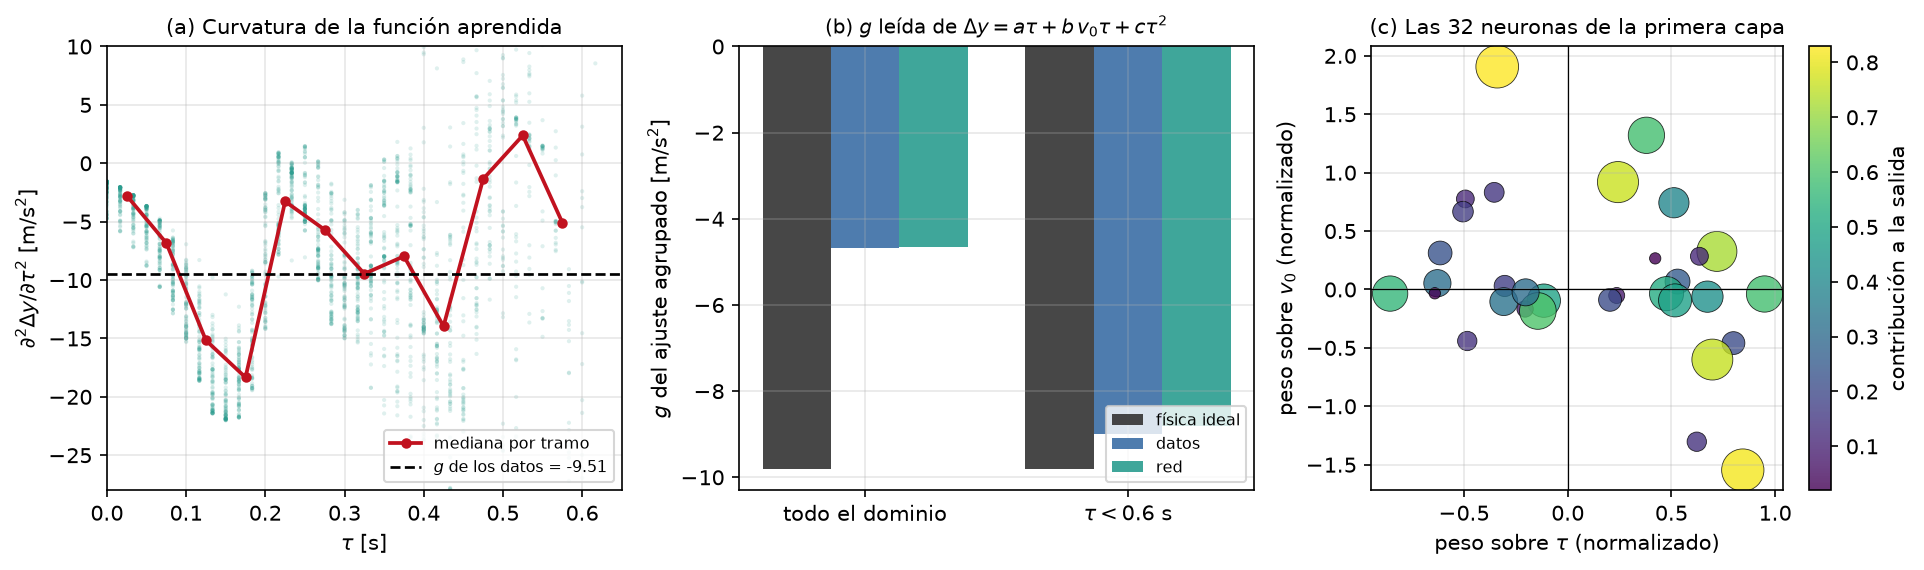
\includegraphics[width=\linewidth]{imgs/06_pesos.png}
  \caption{(a) Segunda derivada de la función aprendida, punto a punto sobre
    los datos de prueba, con su mediana por tramos. Oscila alrededor del valor
    experimental (línea discontinua) en vez de ser constante. (b) $g$ obtenida
    ajustando el modelo de MRUV agrupado a la salida de la red y, como control,
    a los datos experimentales mismos: la red sigue a los datos, no a la física
    ideal. (c) Pesos de entrada de las 32 neuronas de la primera capa; el
    tamaño y el color indican su contribución a la salida.}
  \label{fig:pesos}
\end{figure}

\subsubsection{La ecuación que la red aprendió, contra los datos}

El resultado anterior invita a preguntar si la desviación respecto de la física
ideal es culpa de la red o una propiedad del conjunto de datos. Para
averiguarlo se ajusta el modelo
\begin{equation}
  \Delta y = a\,\tau + b\,v_0\tau + c\,\tau^2
  \label{eq:modelo_agrupado}
\end{equation}
---cuyos coeficientes la física fija en $(0,\,1,\,g/2)$--- tanto a la
superficie de salida de la red como, \textbf{y esto es lo decisivo}, a los
datos experimentales mismos. Sin ese control la comparación no significa nada.

\begin{table}[H]
  \centering
  \begin{tabular}{llrrr}
    \toprule
    Dominio & Fuente & $a$ & $b$ & $2c = g$ \\
    \midrule
    \multirow{3}{*}{Todo ($\num{2843}$ puntos)}
      & Física ideal & $0.000$ & $1.000$ & $-9.810$ \\
      & Datos experimentales & $-0.808$ & $0.814$ & $-4.674$ \\
      & Red $\tanh$ & $-0.979$ & $0.486$ & $\mathbf{-4.657}$ \\
    \midrule
    \multirow{3}{*}{$\tau<\unit{0.6}{\second}$ ($\num{2696}$ puntos)}
      & Física ideal & $0.000$ & $1.000$ & $-9.810$ \\
      & Datos experimentales & $+0.066$ & $1.043$ & $-8.995$ \\
      & Red $\tanh$ & $-0.153$ & $0.647$ & $\mathbf{-8.807}$ \\
    \bottomrule
  \end{tabular}
  \caption{Coeficientes del modelo~\eqref{eq:modelo_agrupado} ajustado a la
    salida de la red y a los datos experimentales, en dos dominios. El
    coeficiente cuadrático de la red sigue al de los datos con una diferencia
    inferior al \SI{2}{\percent} en ambos casos, incluso cuando el de los datos
    se aleja mucho del valor físico.}
  \label{tab:ecuacion}
\end{table}

El resultado es nítido. Sobre todo el dominio, el ajuste agrupado de los
\emph{datos} da $g=\num{-4.67}~\meter\per\second\squared$, muy lejos del valor
físico; la red da $\num{-4.66}$. Restringiendo a $\tau<\unit{0.6}{\second}$ ---
donde vive el \SI{95}{\percent} de las muestras y el ajuste agrupado deja de
estar contaminado por la cola de clips largos, que son pocos y los peor
seguidos--- los datos dan $\num{-9.00}$ y la red $\num{-8.81}$. En los dos
dominios la red reproduce el coeficiente cuadrático de los datos con menos del
\SI{2}{\percent} de diferencia, \emph{sesgos incluidos}.

La conclusión es que la red aprendió lo que el conjunto de datos contiene, no
la ley ideal, y que es fiel a él hasta en sus defectos. Donde sí se aparta es
en el coeficiente $b$, la sensibilidad a la velocidad inicial: la red usa
$b\approx\num{0.65}$ donde los datos piden $\num{1.04}$. Eso es coherente con
lo observado en la sección~\ref{subsec:error} ---que la red supera al modelo
analítico de MRUV--- e indica que no toma $v_0$ al pie de la letra sino que la
descuenta parcialmente, verosímilmente porque la estimación de $v_0$ a partir
de tres puntos es ruidosa.

\subsubsection{Cómo está repartida la representación}

El panel~(c) de la figura~\ref{fig:pesos} muestra los pesos de entrada de las
32 neuronas de la primera capa. No hay ninguna \enquote{neurona de la
gravedad}: las neuronas se reparten por todo el plano $(w_\tau, w_{v_0})$, con
una razón mediana $\abs{w_{v_0}/w_\tau}=\num{0.54}$, y las seis de mayor
contribución a la salida no comparten estructura reconocible. Además, 15 de las
32 operan casi siempre en el régimen lineal de la $\tanh$ (activación con
$\abs{\tanh}>0.9$ en menos del \SI{10}{\percent} del dominio).

Es decir: la parábola no está codificada en ninguna unidad ni en ningún peso
identificable, sino en la \emph{combinación} de muchas neuronas casi lineales,
ninguna de las cuales es interpretable por separado. Ese es, probablemente, el
hallazgo más honesto de esta sección: la red recupera correctamente el
parámetro físico, pero no lo hace construyendo internamente una representación
de la ecuación de movimiento que un físico pueda leer. La física está en el
comportamiento agregado de la red, no en su estructura.

\subsection{Síntesis}

Reuniendo la evidencia:

\begin{itemize}
\item Los datos experimentales contienen la física buscada: ajustados clip por
  clip dan $g_{\text{exp}}=\num{-9.43}~\meter\per\second\squared$
  (tabla~\ref{tab:datos}).
\item La red $\tanh$ profunda con entradas $(\tau,v_0)$ recupera
  $g=\num{-9.46}\pm\num{0.33}~\meter\per\second\squared$ sobre clips no vistos,
  a un \SI{0.2}{\percent} de lo que el método clásico obtiene de esos mismos
  datos (tabla~\ref{tab:g}).
\item Su RMSE de \num{0.142}~\meter\ ($R^2=\num{0.93}$) supera en un
  \SI{30}{\percent} al modelo analítico de MRUV con una única $g$ ajustada
  (tabla~\ref{tab:rmse}).
\item Las predicciones siguen la trayectoria propia de cada clip
  (figura~\ref{fig:tray}), y la distribución de las $g$ predichas se superpone
  con la de los datos (figura~\ref{fig:hist}).
\item El coste de entrenar es lineal en el número de épocas, y el beneficio se
  agota pronto: el RMSE se estanca hacia la época 20 y la mejor estimación de
  $g$ se alcanza hacia la 200 (tabla~\ref{tab:epocas}).
\item Al mirar dentro de la red, el ajuste agrupado de su salida reproduce el
  coeficiente cuadrático de los datos con menos del \SI{2}{\percent} de
  diferencia, pero su curvatura punto a punto no es constante y ninguna neurona
  es interpretable por separado (tablas~\ref{tab:derivadas}
  y~\ref{tab:ecuacion}).
\end{itemize}

\textbf{El supuesto del anteproyecto se verifica:} una red neuronal entrenada
con datos experimentales de caída libre sí permite recuperar el modelo físico
subyacente. Lo que el estudio muestra además es que ese resultado depende
críticamente de cómo se estructuren las entradas: la misma arquitectura, con
los mismos datos y el mismo entrenamiento, entrega o no entrega la gravedad
según que la representación haga identificable el problema.


% % % % % % % % % % % % % % % % % % % % % % % % % % % % % % % % % % %
\section{Limitaciones del estudio}
\label{sec:limitaciones}

Las siguientes son propiedades del conjunto de datos y del procedimiento, y
acotan lo que puede lograrse con ellos, con red o sin ella.

\begin{enumerate}
\item \textbf{Sesgo experimental en $g$.} El método clásico aplicado a estos
  datos da $\num{-9.43}~\meter\per\second\squared$, un \SI{3.9}{\percent} por
  debajo del valor físico. Ese sesgo ---probablemente de calibración de la
  escala espacial o de la velocidad de fotogramas--- afecta por igual a la red
  y al ajuste clásico, y fija el techo de exactitud alcanzable con este
  conjunto.

\item \textbf{Calidad de la digitalización.} La dispersión de
  $\num{1.82}~\meter\per\second\squared$ en la $g$ experimental por clip indica
  cuantización a nivel de píxel en el seguimiento. El filtro de calidad
  descarta los peores casos, pero no elimina el ruido de fondo, que se refleja
  en el residuo mediano de \unit{3.4}{\centi\meter}.

\item \textbf{Duración de los clips.} Con \unit{0.53}{\second} de media, el
  término cuadrático de la ecuación~\eqref{eq:mruv_ref} contribuye poco frente
  al ruido de medición, lo que hace intrínsecamente difícil estimar $g$ a
  partir de un clip aislado.

\item \textbf{Estimación de $v_0$.} Se obtiene de los tres primeros puntos de
  cada clip y arrastra el ruido de esas mediciones. Que la red supere al modelo
  analítico de MRUV (sección~\ref{subsec:error}) sugiere que compensa un sesgo
  de esa estimación, pero no se comprobó de forma directa.

\item \textbf{La física no es legible en la estructura de la red.} Como muestra
  la sección~\ref{subsec:pesos}, la red recupera $g$ correctamente pero su
  curvatura punto a punto no es constante y la representación está repartida
  entre muchas neuronas casi lineales, ninguna interpretable por separado. La
  inspección permite afirmar qué \emph{no} hay dentro de la red, pero no
  extraer de ella una forma cerrada del modelo físico.

\item \textbf{El criterio de parada se apoya en el error de predicción.} La
  sección~\ref{subsec:epocas} muestra que el RMSE y el error en $g$ no son
  monótonos entre sí, de modo que la parada temprana sobre el error de
  validación no garantiza detenerse en el óptimo del parámetro físico. En este
  problema coincidieron aproximadamente, pero eso no es general.
\end{enumerate}


% % % % % % % % % % % % % % % % % % % % % % % % % % % % % % % % % % %
\section{Conclusiones}
\label{sec:conclusiones}

\begin{enumerate}
\item Se construyó un conjunto de datos experimental propio de caída libre: 609
  clips grabados a \unit{60}{\hertz}, 606 utilizables y 581 tras el filtro de
  calidad, con \num{18\,992} pares $(t,y)$ digitalizados con \emph{Tracker}. El
  conjunto contiene la física buscada: un ajuste cuadrático clip por clip
  recupera $g=\num{-9.43}~\meter\per\second\squared$, a un \SI{3.9}{\percent}
  del valor esperado.

\item Se implementaron y entrenaron en PyTorch tres arquitecturas de red
  neuronal de capacidad creciente, bajo tres formulaciones de las entradas y
  con cinco semillas cada una, con partición por clip completo, parada temprana
  y tres líneas base clásicas. Con ello se cumplieron los objetivos específicos
  relativos a la construcción, entrenamiento y estudio de redes neuronales.

\item \textbf{El supuesto del anteproyecto se verifica.} Con entradas
  $(\tau,v_0)$ y salida $\Delta y$, la red $\tanh$ profunda recupera
  $g=\num{-9.46}\pm\num{0.33}~\meter\per\second\squared$ sobre clips que no vio
  durante el entrenamiento. Frente al $\num{-9.48}~\meter\per\second\squared$
  que el método clásico extrae de esos mismos datos, la discrepancia es del
  \SI{0.2}{\percent}. La diferencia restante con $\num{-9.81}$ es sesgo
  experimental, no fallo del modelo.

\item En términos de predicción, la red alcanza RMSE~$=\num{0.142}~\meter$ y
  $R^2=\num{0.93}$ sobre clips no vistos, frente a los \num{0.553}~\meter\ del
  predictor constante.

\item \textbf{La red supera al modelo analítico.} RMSE de \num{0.142}~\meter\
  frente a \num{0.202}~\meter\ de la ecuación de MRUV con una única $g$
  ajustada, con las mismas entradas. Es el punto del proyecto en que la red
  aporta algo que el método clásico no proporciona, verosímilmente por
  compensar el sesgo de la estimación de $v_0$.

\item \textbf{La representación de las entradas y la capacidad de la red son
  dos límites distintos y sucesivos.} Con la formulación directa, multiplicar
  por 165 el número de parámetros no mejora la estimación de $g$; con la
  formulación completa, la misma escalada la lleva de $\num{-4.68}$ a
  $\num{-9.46}~\meter\per\second\squared$. Cuando el límite es de información,
  ninguna arquitectura lo supera; cuando es de representación, la capacidad
  pasa a ser decisiva.

\item \textbf{El beneficio de entrenar más se agota mucho antes que el coste.}
  El tiempo crece linealmente con las épocas, mientras que el RMSE alcanza su
  valor final hacia la época 20 y la mejor estimación de $g$ hacia la 200. Para
  esta red y estos datos el punto de operación razonable son 100--200 épocas,
  unos \SI{2}{\second} de cómputo; las 600 épocas siguientes cuadruplican el
  tiempo y no mejoran nada.

\item \textbf{El error de predicción y la recuperación de la física no van al
  mismo ritmo, y pueden ir en sentidos opuestos.} La red media $(4)$ mejora su
  RMSE de \num{0.167} a \num{0.157}~\meter\ entre las épocas 10 y 800 mientras
  su error en $g$ empeora del \SI{17.7}{\percent} al \SI{29.1}{\percent}. Un
  criterio de parada basado únicamente en el error de validación no garantiza,
  por tanto, detenerse donde el parámetro físico es mejor.

\item \textbf{La red aprende lo que los datos contienen, con sus sesgos.} Al
  ajustar el modelo $\Delta y = a\tau + b\,v_0\tau + c\tau^2$ a la salida de la
  red y, como control, a los datos experimentales, el coeficiente cuadrático de
  la red sigue al de los datos con menos del \SI{2}{\percent} de diferencia en
  los dos dominios examinados, incluso donde el de los datos se aparta mucho
  del valor físico.

\item \textbf{La física está en el comportamiento de la red, no en su
  estructura.} La curvatura de la función aprendida tiene el signo y el orden
  de magnitud correctos pero no es constante, y la representación está
  repartida entre muchas neuronas casi lineales sin que ninguna sea
  interpretable por separado. La red recupera $g$ correctamente sin construir
  internamente nada que se parezca a la ecuación de movimiento. Extraer una
  forma cerrada exigiría arquitecturas diseñadas para ello, y esa es la
  continuación natural del trabajo.

\item Una red neuronal entrenada con MSE converge a la media condicional de los
  datos. Que esa media condicional coincida o no con la ley física depende
  enteramente de cómo se hayan estructurado las entradas: la condición de
  identificabilidad es previa a cualquier consideración de arquitectura. Este
  es el aprendizaje central del proyecto y la base sobre la que se plantea su
  continuación.

\item Desde el punto de vista metodológico, la validación de un modelo de
  aprendizaje automático contra una teoría física exige que el valor de
  referencia se verifique con el mismo rigor que el valor predicho. Aquí eso
  significó estimar $g$ \emph{clip por clip} en ambos lados de la comparación y
  contrastar el resultado contra líneas base clásicas explícitas.
\end{enumerate}


% % % % % % % % % % % % % % % % % % % % % % % % % % % % % % % % % % %
\section{Trabajo futuro}
\label{sec:trabajofuturo}

Las siguientes líneas quedan abiertas, ordenadas de la más inmediata a la más
ambiciosa, y constituyen la continuación natural hacia el EPS.

\paragraph{Cerrar la brecha con el oráculo.} La red alcanza
RMSE~$=\num{0.142}~\meter$ frente a los $\num{0.040}~\meter$ del ajuste por
clip. Parte de esa diferencia es irreducible ---el oráculo dispone de tres
parámetros por clip--- pero conviene medir cuánta. Dos vías: predecir
directamente los coeficientes $(c_0,c_1,c_2)$ de cada clip en lugar de puntos
sueltos, y estimar $v_0$ con más robustez (ajuste local en vez de tres puntos).

\paragraph{Diagnosticar el sesgo experimental.} El método clásico da
$\num{-9.43}~\meter\per\second\squared$ sobre estos datos, un
\SI{3.9}{\percent} por debajo del valor real. Antes de perseguir mejoras en el
modelo conviene identificar si el sesgo viene de la calibración de la escala
espacial, de la velocidad de fotogramas declarada o del arrastre del aire, y
corregirlo en la toma de datos.

\paragraph{Mejorar la calidad de los datos.} Grabar clips más largos o desde
mayor altura, para que el término cuadrático domine sobre el ruido, y aumentar
la resolución espacial o la frecuencia de muestreo. Con
\unit{0.53}{\second} de media por clip, la señal cuadrática es débil frente a
la cuantización de píxel.

\paragraph{Hacer la red interpretable a propósito.} La inspección de la
sección~\ref{subsec:pesos} muestra que la física no está codificada de forma
legible en los pesos. Si se quiere que lo esté hay que forzarlo: redes con una
capa de cuello de botella de una sola unidad, activaciones polinómicas, o
regresión simbólica sobre la función aprendida. Cualquiera de las tres
convertiría \enquote{la red predice bien} en \enquote{la red entrega una
ecuación}, que es el objetivo natural del EPS.

\paragraph{Un criterio de parada basado en la física.} Como el error de
predicción y el error en $g$ no son monótonos entre sí
(sección~\ref{subsec:epocas}), tiene sentido explorar una parada temprana que
vigile directamente la $g$ estimada sobre los clips de validación en lugar del
MSE.

\paragraph{Explorar el aprendizaje con restricciones físicas.} Incorporar el
residuo de la ecuación de movimiento a la función de coste (\emph{physics-informed
neural networks}) permitiría comparar cuánta física aporta la arquitectura
frente a cuánta aporta la función de coste, y previsiblemente reducir la
dispersión entre semillas.

\paragraph{Generalizar a otros marcos teóricos.} Con el protocolo ya validado
sobre la caída libre, extender el estudio a movimiento en dos dimensiones, a
sistemas con fricción y a osciladores, que es el objetivo planteado para el
EPS. El procedimiento desarrollado aquí ---formular el problema de modo que sea
identificable, comparar contra una línea base clásica y estimar el parámetro
físico caso por caso--- es directamente transferible a esos sistemas.


% % % % % % % % % % % % % % % % % % % % % % % % % % % % % % % % % % %
\section{Bibliografía}
\label{sec:biografia}

\subsection*{Referencias comentadas}
\label{sec:referencias}

Todo lo pertinente a teoría física fue tomado de Blatt~\cite{Fisica}. La
referencia estadística predeterminada, para regresión, mínimos cuadrados y
métricas de error, es el libro de Triola~\cite{triola_2018_estadstica}. La parte
matemática --- derivadas parciales y regla de la cadena --- se consultó en el
libro de cálculo de Zill~\cite{zill_1985_clculo}. El canal de YouTube DotCSV es
una referencia audiovisual bastante completa en cuanto a redes neuronales se
refiere~\cite{santana_2018_1,santana_2018_2,santana_2018_3,santana_2018_3_5}, y
complementa la introducción de Antonio~\cite{antonio_2023_introduccin} y la
documentación divulgativa de IBM~\cite{ibm_qu}. Para consultas técnicas rápidas
sobre funciones de activación se usó la página de Wikipedia
correspondiente~\cite{wikipediacontributors_2018_activation}. Las ayudas para
entender el manejo de bibliotecas de aprendizaje profundo se tomaron de Kapoor,
Gulli y Pal~\cite{Amita} y, como documentación complementaria, del libro de
Martínez~\cite{Jesus}. La documentación de TensorFlow~\cite{TensorFlow} se
consultó durante la fase inicial, antes de la migración a PyTorch descrita en
la sección~\ref{subsec:ts}.

\bibliographystyle{ieeetr}
\bibliography{referencias}
\end{document}


%%% Local Variables:
%%% mode: latex
%%% TeX-master: t
%%% End:
